% Options for packages loaded elsewhere
\PassOptionsToPackage{unicode}{hyperref}
\PassOptionsToPackage{hyphens}{url}
%
\documentclass[
]{article}
\usepackage{lmodern}
\usepackage{amssymb,amsmath}
\usepackage{ifxetex,ifluatex}
\ifnum 0\ifxetex 1\fi\ifluatex 1\fi=0 % if pdftex
  \usepackage[T1]{fontenc}
  \usepackage[utf8]{inputenc}
  \usepackage{textcomp} % provide euro and other symbols
\else % if luatex or xetex
  \usepackage{unicode-math}
  \defaultfontfeatures{Scale=MatchLowercase}
  \defaultfontfeatures[\rmfamily]{Ligatures=TeX,Scale=1}
\fi
% Use upquote if available, for straight quotes in verbatim environments
\IfFileExists{upquote.sty}{\usepackage{upquote}}{}
\IfFileExists{microtype.sty}{% use microtype if available
  \usepackage[]{microtype}
  \UseMicrotypeSet[protrusion]{basicmath} % disable protrusion for tt fonts
}{}
\makeatletter
\@ifundefined{KOMAClassName}{% if non-KOMA class
  \IfFileExists{parskip.sty}{%
    \usepackage{parskip}
  }{% else
    \setlength{\parindent}{0pt}
    \setlength{\parskip}{6pt plus 2pt minus 1pt}}
}{% if KOMA class
  \KOMAoptions{parskip=half}}
\makeatother
\usepackage{xcolor}
\IfFileExists{xurl.sty}{\usepackage{xurl}}{} % add URL line breaks if available
\IfFileExists{bookmark.sty}{\usepackage{bookmark}}{\usepackage{hyperref}}
\hypersetup{
  pdftitle={DDS Project1: Budwieser Case Study},
  pdfauthor={Bgaither,Alarsen,Amejia},
  hidelinks,
  pdfcreator={LaTeX via pandoc}}
\urlstyle{same} % disable monospaced font for URLs
\usepackage[margin=1in]{geometry}
\usepackage{color}
\usepackage{fancyvrb}
\newcommand{\VerbBar}{|}
\newcommand{\VERB}{\Verb[commandchars=\\\{\}]}
\DefineVerbatimEnvironment{Highlighting}{Verbatim}{commandchars=\\\{\}}
% Add ',fontsize=\small' for more characters per line
\usepackage{framed}
\definecolor{shadecolor}{RGB}{248,248,248}
\newenvironment{Shaded}{\begin{snugshade}}{\end{snugshade}}
\newcommand{\AlertTok}[1]{\textcolor[rgb]{0.94,0.16,0.16}{#1}}
\newcommand{\AnnotationTok}[1]{\textcolor[rgb]{0.56,0.35,0.01}{\textbf{\textit{#1}}}}
\newcommand{\AttributeTok}[1]{\textcolor[rgb]{0.77,0.63,0.00}{#1}}
\newcommand{\BaseNTok}[1]{\textcolor[rgb]{0.00,0.00,0.81}{#1}}
\newcommand{\BuiltInTok}[1]{#1}
\newcommand{\CharTok}[1]{\textcolor[rgb]{0.31,0.60,0.02}{#1}}
\newcommand{\CommentTok}[1]{\textcolor[rgb]{0.56,0.35,0.01}{\textit{#1}}}
\newcommand{\CommentVarTok}[1]{\textcolor[rgb]{0.56,0.35,0.01}{\textbf{\textit{#1}}}}
\newcommand{\ConstantTok}[1]{\textcolor[rgb]{0.00,0.00,0.00}{#1}}
\newcommand{\ControlFlowTok}[1]{\textcolor[rgb]{0.13,0.29,0.53}{\textbf{#1}}}
\newcommand{\DataTypeTok}[1]{\textcolor[rgb]{0.13,0.29,0.53}{#1}}
\newcommand{\DecValTok}[1]{\textcolor[rgb]{0.00,0.00,0.81}{#1}}
\newcommand{\DocumentationTok}[1]{\textcolor[rgb]{0.56,0.35,0.01}{\textbf{\textit{#1}}}}
\newcommand{\ErrorTok}[1]{\textcolor[rgb]{0.64,0.00,0.00}{\textbf{#1}}}
\newcommand{\ExtensionTok}[1]{#1}
\newcommand{\FloatTok}[1]{\textcolor[rgb]{0.00,0.00,0.81}{#1}}
\newcommand{\FunctionTok}[1]{\textcolor[rgb]{0.00,0.00,0.00}{#1}}
\newcommand{\ImportTok}[1]{#1}
\newcommand{\InformationTok}[1]{\textcolor[rgb]{0.56,0.35,0.01}{\textbf{\textit{#1}}}}
\newcommand{\KeywordTok}[1]{\textcolor[rgb]{0.13,0.29,0.53}{\textbf{#1}}}
\newcommand{\NormalTok}[1]{#1}
\newcommand{\OperatorTok}[1]{\textcolor[rgb]{0.81,0.36,0.00}{\textbf{#1}}}
\newcommand{\OtherTok}[1]{\textcolor[rgb]{0.56,0.35,0.01}{#1}}
\newcommand{\PreprocessorTok}[1]{\textcolor[rgb]{0.56,0.35,0.01}{\textit{#1}}}
\newcommand{\RegionMarkerTok}[1]{#1}
\newcommand{\SpecialCharTok}[1]{\textcolor[rgb]{0.00,0.00,0.00}{#1}}
\newcommand{\SpecialStringTok}[1]{\textcolor[rgb]{0.31,0.60,0.02}{#1}}
\newcommand{\StringTok}[1]{\textcolor[rgb]{0.31,0.60,0.02}{#1}}
\newcommand{\VariableTok}[1]{\textcolor[rgb]{0.00,0.00,0.00}{#1}}
\newcommand{\VerbatimStringTok}[1]{\textcolor[rgb]{0.31,0.60,0.02}{#1}}
\newcommand{\WarningTok}[1]{\textcolor[rgb]{0.56,0.35,0.01}{\textbf{\textit{#1}}}}
\usepackage{graphicx,grffile}
\makeatletter
\def\maxwidth{\ifdim\Gin@nat@width>\linewidth\linewidth\else\Gin@nat@width\fi}
\def\maxheight{\ifdim\Gin@nat@height>\textheight\textheight\else\Gin@nat@height\fi}
\makeatother
% Scale images if necessary, so that they will not overflow the page
% margins by default, and it is still possible to overwrite the defaults
% using explicit options in \includegraphics[width, height, ...]{}
\setkeys{Gin}{width=\maxwidth,height=\maxheight,keepaspectratio}
% Set default figure placement to htbp
\makeatletter
\def\fps@figure{htbp}
\makeatother
\setlength{\emergencystretch}{3em} % prevent overfull lines
\providecommand{\tightlist}{%
  \setlength{\itemsep}{0pt}\setlength{\parskip}{0pt}}
\setcounter{secnumdepth}{-\maxdimen} % remove section numbering

\title{DDS Project1: Budwieser Case Study}
\author{Bgaither,Alarsen,Amejia}
\date{2/11/2020}

\begin{document}
\maketitle

\textbf{Introduction}

\textbf{The Purpose of this analysis is to explore and present to the
leadership of Budwieser the following findings:}

\textbf{The number of breweries per state in the United States.}
\textbf{If there is any type of linear relationship to IBU
(International Bitterness Unit) and ABV (Alcohol by Volume).}
\textbf{Explores if there is a difference with respect to IBU and ABV
between IPAs (India Pale Ales) and other types of Ale using two
different classification techniques.} \textbf{If there is a difference
in the ABV in different regions of the United States.} \textbf{If there
is a difference in the IBU for the 12 OZ. and 16 OZ. serving sizes.}

\textbf{This document will address the previously stated questions as
well as provide the research methodolgy and address assumptions about
the data.}

Loading Data into R environment as well as loading the following
libraries: ggplot2, car, dplyr, stringr, maps, ggpubr Coercing the
`state' column in the US states spatial data to a character to be used
downstream

\begin{Shaded}
\begin{Highlighting}[]
\KeywordTok{library}\NormalTok{(ggplot2)}
\KeywordTok{library}\NormalTok{(car)}
\KeywordTok{library}\NormalTok{(dplyr)}
\KeywordTok{library}\NormalTok{(stringr)}
\KeywordTok{library}\NormalTok{(maps)}
\KeywordTok{library}\NormalTok{(ggpubr)}

\NormalTok{dfBeers =}\StringTok{ }\KeywordTok{read.csv}\NormalTok{(}\StringTok{"C:/Users/BGaither/Documents/GitHub/DS_6306/RawDataFiles/Beers.csv"}\NormalTok{,}\DataTypeTok{header =} \OtherTok{TRUE}\NormalTok{)}

\NormalTok{dfBreweries =}\StringTok{ }\KeywordTok{read.csv}\NormalTok{(}\StringTok{"C:/Users/BGaither/Documents/GitHub/DS_6306/RawDataFiles/Breweries.csv"}\NormalTok{,}\DataTypeTok{header =} \OtherTok{TRUE}\NormalTok{)}

\NormalTok{us_states =}\StringTok{ }\KeywordTok{read.csv}\NormalTok{(}\StringTok{'C:/Users/BGaither/Documents/GitHub/DS_6306/RawDataFiles/states.csv'}\NormalTok{, }\DataTypeTok{header =} \OtherTok{TRUE}\NormalTok{)}

\CommentTok{#dfBeers = read.csv(file.choose(),header = TRUE)}

\CommentTok{#dfBreweries = read.csv(file.choose(),header = TRUE)}

\CommentTok{#us_states = read.csv(file.choose(), header = TRUE)}



\NormalTok{us_states[}\StringTok{'state'}\NormalTok{] =}\StringTok{ }\KeywordTok{as.character}\NormalTok{(us_states}\OperatorTok{$}\NormalTok{state)}
\CommentTok{#head(dfBeers)}
\CommentTok{#head(dfBreweries)}
\end{Highlighting}
\end{Shaded}

\textbf{Question of interest: How many breweries are present in each
state?}

\textbf{Answer:} \textbf{The states with the largest amounts of
breweries are Colorado, California and Michigan. The states with the
fewest amounts of breweries are North Dakota, South Dakota and West
Virginia. The states with the largest amounts of breweries tend to be
states with moderate to high populations that have strong craft brew
scenes. The states with the fewest amounts of breweries tend to be lower
population, rural states.}

\begin{Shaded}
\begin{Highlighting}[]
\CommentTok{#}
\KeywordTok{data.frame}\NormalTok{(}\KeywordTok{table}\NormalTok{(dfBreweries}\OperatorTok{$}\NormalTok{State)) }\OperatorTok\StringTok{ }\KeywordTok{ggplot}\NormalTok{(}\KeywordTok{aes}\NormalTok{(}\DataTypeTok{x =}\NormalTok{ State, }\DataTypeTok{y =}\NormalTok{ Freq), }\DataTypeTok{mapping=}\KeywordTok{aes}\NormalTok{(}\DataTypeTok{x =} \KeywordTok{reorder}\NormalTok{(Var1, }\OperatorTok{-}\NormalTok{Freq), }\DataTypeTok{y =}\NormalTok{ Freq)) }\OperatorTok{+}\StringTok{ }\KeywordTok{geom_bar}\NormalTok{(}\DataTypeTok{stat =} \StringTok{"Identity"}\NormalTok{, }\DataTypeTok{fill=}\StringTok{"blue"}\NormalTok{) }\OperatorTok{+}\StringTok{ }\KeywordTok{xlab}\NormalTok{(}\StringTok{"State"}\NormalTok{) }\OperatorTok{+}\StringTok{ }\KeywordTok{ylab}\NormalTok{(}\StringTok{"Count"}\NormalTok{) }\OperatorTok{+}\StringTok{ }\KeywordTok{ggtitle}\NormalTok{(}\StringTok{"Number of Breweries by State"}\NormalTok{)}
\end{Highlighting}
\end{Shaded}

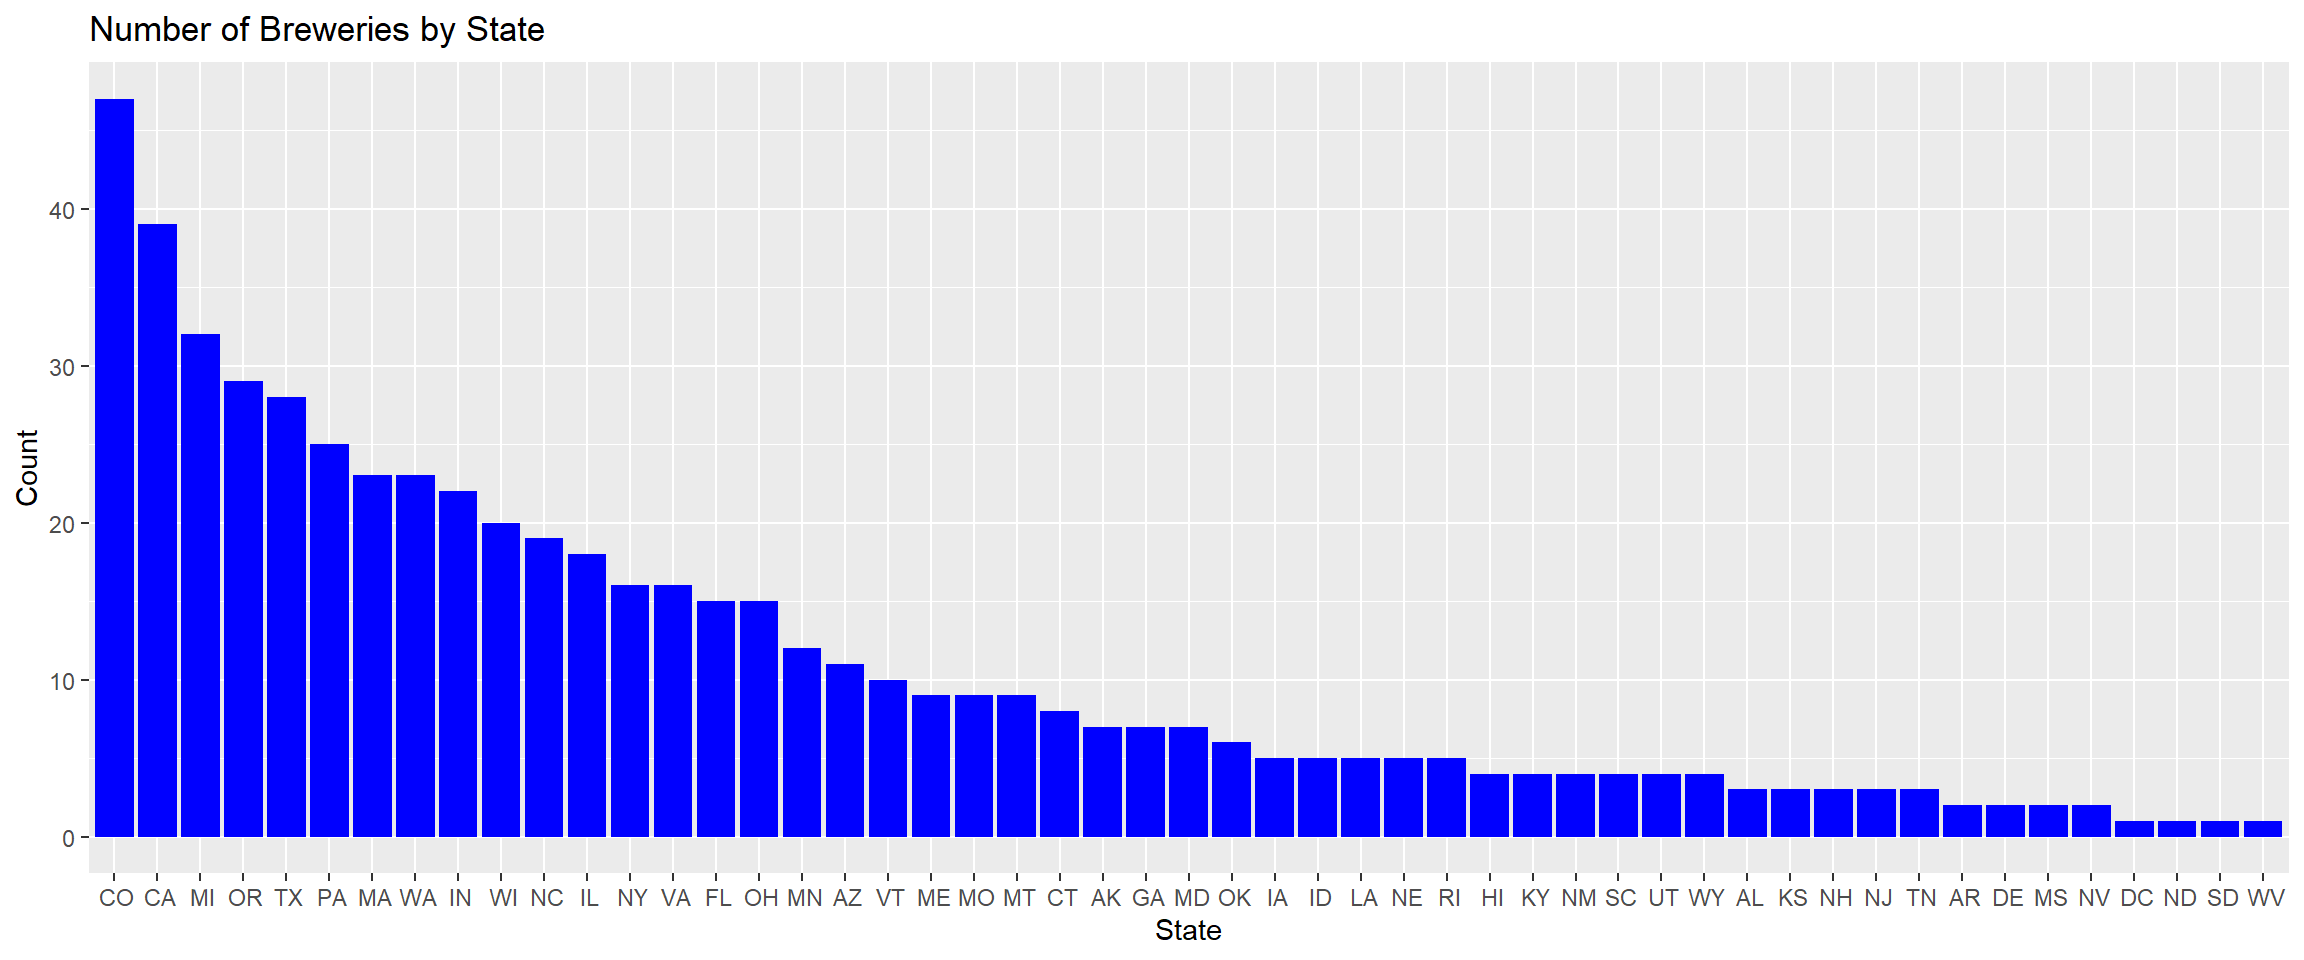
\includegraphics{Beer_Study_files/figure-latex/unnamed-chunk-2-1.pdf}

\begin{Shaded}
\begin{Highlighting}[]
\CommentTok{#}
\end{Highlighting}
\end{Shaded}

Let's use the data above to determine how the states make up the total
cumulative percent of all breweries using a Pareto Analysis

\begin{Shaded}
\begin{Highlighting}[]
\NormalTok{myDF =}\StringTok{ }\NormalTok{dfBreweries }\OperatorTok\StringTok{ }\KeywordTok{count}\NormalTok{(dfBreweries}\OperatorTok{$}\NormalTok{State)}
\CommentTok{#descending sort}
\NormalTok{myDF <-}\StringTok{ }\NormalTok{myDF[}\KeywordTok{order}\NormalTok{(myDF}\OperatorTok{$}\NormalTok{n, }\DataTypeTok{decreasing =} \OtherTok{TRUE}\NormalTok{),]}
\CommentTok{#adding a cumulative sum}
\NormalTok{myDF}\OperatorTok{$}\NormalTok{cumulative <-}\StringTok{ }\KeywordTok{cumsum}\NormalTok{(myDF}\OperatorTok{$}\NormalTok{n)}
\KeywordTok{colnames}\NormalTok{(myDF) <-}\StringTok{ }\KeywordTok{c}\NormalTok{(}\StringTok{"State"}\NormalTok{, }\StringTok{"Count"}\NormalTok{, }\StringTok{"Cumulative"}\NormalTok{)}

\KeywordTok{library}\NormalTok{(ggQC)}

\KeywordTok{ggplot}\NormalTok{(myDF, }\KeywordTok{aes}\NormalTok{(}\DataTypeTok{x=}\KeywordTok{reorder}\NormalTok{(State, }\OperatorTok{-}\NormalTok{Count), }\DataTypeTok{y=}\NormalTok{Count)) }\OperatorTok{+}\StringTok{ }\KeywordTok{geom_bar}\NormalTok{(}\DataTypeTok{stat=}\StringTok{"identity"}\NormalTok{) }\OperatorTok{+}\StringTok{ }\KeywordTok{theme}\NormalTok{(}\DataTypeTok{axis.text.x=}\KeywordTok{element_text}\NormalTok{(}\DataTypeTok{angle=}\DecValTok{90}\NormalTok{,}\DataTypeTok{hjust=}\DecValTok{1}\NormalTok{)) }\OperatorTok{+}\StringTok{ }\KeywordTok{stat_pareto}\NormalTok{(}\DataTypeTok{point.color=}\StringTok{"red"}\NormalTok{, }\DataTypeTok{point.size=}\DecValTok{2}\NormalTok{, }\DataTypeTok{line.color=}\StringTok{"black"}\NormalTok{, }\DataTypeTok{bars.fill =} \KeywordTok{c}\NormalTok{(}\StringTok{"blue"}\NormalTok{, }\StringTok{"orange"}\NormalTok{))}\OperatorTok{+}\StringTok{ }\KeywordTok{labs}\NormalTok{(}\DataTypeTok{title =} \StringTok{"Pareto of Breweries by State"}\NormalTok{, }\DataTypeTok{x=}\StringTok{'States'}\NormalTok{, }\DataTypeTok{y=}\StringTok{'Count'}\NormalTok{)}
\end{Highlighting}
\end{Shaded}

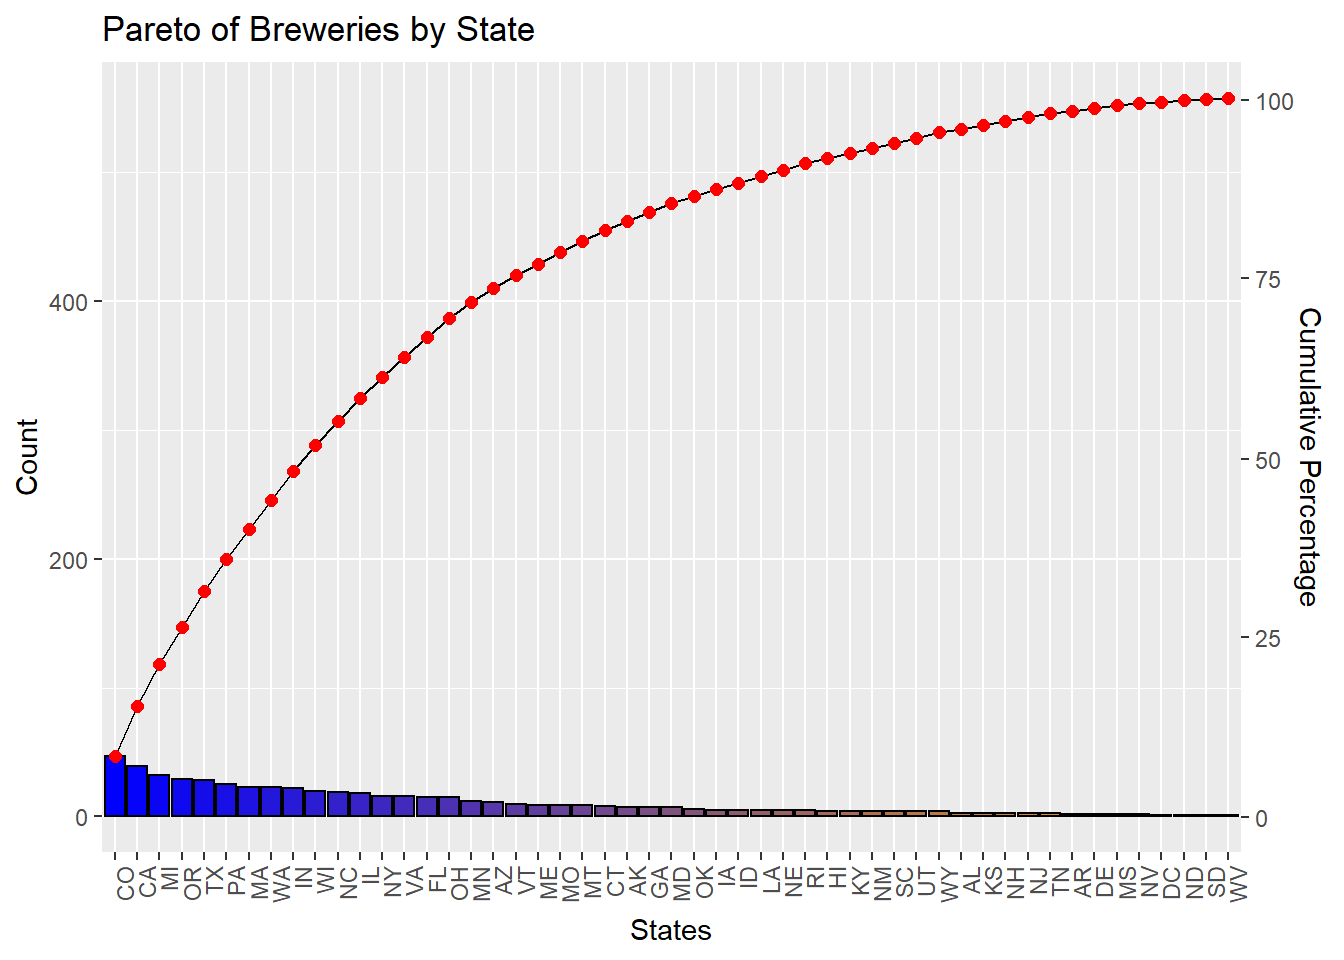
\includegraphics{Beer_Study_files/figure-latex/unnamed-chunk-3-1.pdf}

Merge the individual data frames such that the data set to be used in
the analysis

\begin{Shaded}
\begin{Highlighting}[]
\NormalTok{dfFull =}\StringTok{ }\KeywordTok{left_join}\NormalTok{(dfBeers, dfBreweries, }\DataTypeTok{by=} \KeywordTok{c}\NormalTok{(}\StringTok{"Brewery_id"}\NormalTok{=}\StringTok{"Brew_ID"}\NormalTok{))}
\NormalTok{dfFull[}\StringTok{'State'}\NormalTok{] =}\StringTok{ }\KeywordTok{as.character}\NormalTok{(}\KeywordTok{str_trim}\NormalTok{(dfFull}\OperatorTok{$}\NormalTok{State))}
\NormalTok{dfFull =}\StringTok{ }\KeywordTok{left_join}\NormalTok{(dfFull, us_states, }\DataTypeTok{by =} \KeywordTok{c}\NormalTok{(}\StringTok{"State"}\NormalTok{ =}\StringTok{ "state"}\NormalTok{))}
\CommentTok{#head(dfFull)}
\CommentTok{#tail(dfFull)}
\CommentTok{#dfFull %>% filter(!is.na(IBU))}
\CommentTok{#to evaluate IPAs against Ales}
\NormalTok{dfFull[}\StringTok{"Ales"}\NormalTok{] =}\StringTok{ }\KeywordTok{ifelse}\NormalTok{(}\KeywordTok{grepl}\NormalTok{(}\StringTok{"IPA"}\NormalTok{, dfFull}\OperatorTok{$}\NormalTok{Style),}\StringTok{"IPA"}\NormalTok{, }\KeywordTok{ifelse}\NormalTok{(}\KeywordTok{grepl}\NormalTok{(}\StringTok{"Ale"}\NormalTok{, dfFull}\OperatorTok{$}\NormalTok{Style),}\StringTok{"Ale"}\NormalTok{,}\StringTok{"Other"}\NormalTok{))}
\NormalTok{dfFull}\OperatorTok{$}\NormalTok{Ales =}\StringTok{ }\KeywordTok{as.factor}\NormalTok{(dfFull}\OperatorTok{$}\NormalTok{Ales)}
\end{Highlighting}
\end{Shaded}

Formatting the dataframe

\begin{Shaded}
\begin{Highlighting}[]
\CommentTok{#rename the columns for beer and brewery name}
\NormalTok{dfFull =}\StringTok{ }\NormalTok{dfFull }\OperatorTok\StringTok{ }\KeywordTok{rename}\NormalTok{(}\DataTypeTok{Beer_Name =}\NormalTok{ Name.x, }\DataTypeTok{Brewery_Name =}\NormalTok{ Name.y)}
\CommentTok{#checking to see which columns have NA's}
\KeywordTok{colnames}\NormalTok{(dfFull)[}\KeywordTok{colSums}\NormalTok{(}\KeywordTok{is.na}\NormalTok{(dfFull))}\OperatorTok{>}\DecValTok{0}\NormalTok{]}
\end{Highlighting}
\end{Shaded}

\begin{verbatim}
## [1] "ABV" "IBU"
\end{verbatim}

\textbf{Question of Interest: How many missing values are in the dataset
for ABV and IBU?} \textbf{There are 62 Missing values for ABV and 1005
Missing values for IBU}

\begin{Shaded}
\begin{Highlighting}[]
\KeywordTok{print}\NormalTok{(}\KeywordTok{dim}\NormalTok{(dfFull[}\KeywordTok{is.na}\NormalTok{(dfFull}\OperatorTok{$}\NormalTok{ABV),])[}\DecValTok{1}\NormalTok{]) }
\end{Highlighting}
\end{Shaded}

\begin{verbatim}
## [1] 62
\end{verbatim}

\begin{Shaded}
\begin{Highlighting}[]
\KeywordTok{print}\NormalTok{(}\KeywordTok{dim}\NormalTok{(dfFull[}\KeywordTok{is.na}\NormalTok{(dfFull}\OperatorTok{$}\NormalTok{IBU),])[}\DecValTok{1}\NormalTok{])}
\end{Highlighting}
\end{Shaded}

\begin{verbatim}
## [1] 1005
\end{verbatim}

\textbf{Question of Interest: Which state has the maximum alcoholic
(ABV) beer? Which state has the most bitter (IBU) beer after computing
the median IBU and ABV?}

\textbf{Answer:} \textbf{Looking at Median Alcohol by Volume by State
and Median IBU's by State, the median ABV is highest in DC, Kentucky and
Maine, while ABV tends to be lowest in Wyoming, New Jersey and Utah.
Utah has a maximum ABV for beer, so its lower median ABV makes sense.
The highest median IBU is in Maine, West Virginia and Florida. The
lowest median IBU is in Arizona, Kansas and Wisconsin.}

\begin{Shaded}
\begin{Highlighting}[]
\NormalTok{dfIBU =}\StringTok{ }\NormalTok{dfFull }\OperatorTok\StringTok{ }\KeywordTok{filter}\NormalTok{(}\OperatorTok{!}\KeywordTok{is.na}\NormalTok{(IBU))}
\NormalTok{dfABV =}\StringTok{ }\NormalTok{dfFull }\OperatorTok\StringTok{ }\KeywordTok{filter}\NormalTok{(}\OperatorTok{!}\KeywordTok{is.na}\NormalTok{(ABV))}
\KeywordTok{ggplot}\NormalTok{(}\DataTypeTok{data=}\KeywordTok{aggregate}\NormalTok{(dfABV}\OperatorTok{$}\NormalTok{ABV, }\DataTypeTok{by=}\KeywordTok{list}\NormalTok{(dfABV}\OperatorTok{$}\NormalTok{State), }\DataTypeTok{FUN=}\NormalTok{median), }\DataTypeTok{mapping=}\KeywordTok{aes}\NormalTok{(}\DataTypeTok{x =} \KeywordTok{reorder}\NormalTok{(Group}\FloatTok{.1}\NormalTok{,}\OperatorTok{-}\NormalTok{x), }\DataTypeTok{y =}\NormalTok{ x)) }\OperatorTok{+}\StringTok{ }\KeywordTok{geom_bar}\NormalTok{(}\DataTypeTok{stat =} \StringTok{"identity"}\NormalTok{, }\DataTypeTok{fill=}\StringTok{"blue"}\NormalTok{) }\OperatorTok{+}\StringTok{ }\KeywordTok{xlab}\NormalTok{(}\StringTok{"State"}\NormalTok{) }\OperatorTok{+}\StringTok{ }\KeywordTok{ylab}\NormalTok{(}\StringTok{"ABV"}\NormalTok{) }\OperatorTok{+}\StringTok{ }\KeywordTok{ggtitle}\NormalTok{(}\StringTok{"Median Alcohol By Volume (ABV) by State"}\NormalTok{)}
\end{Highlighting}
\end{Shaded}

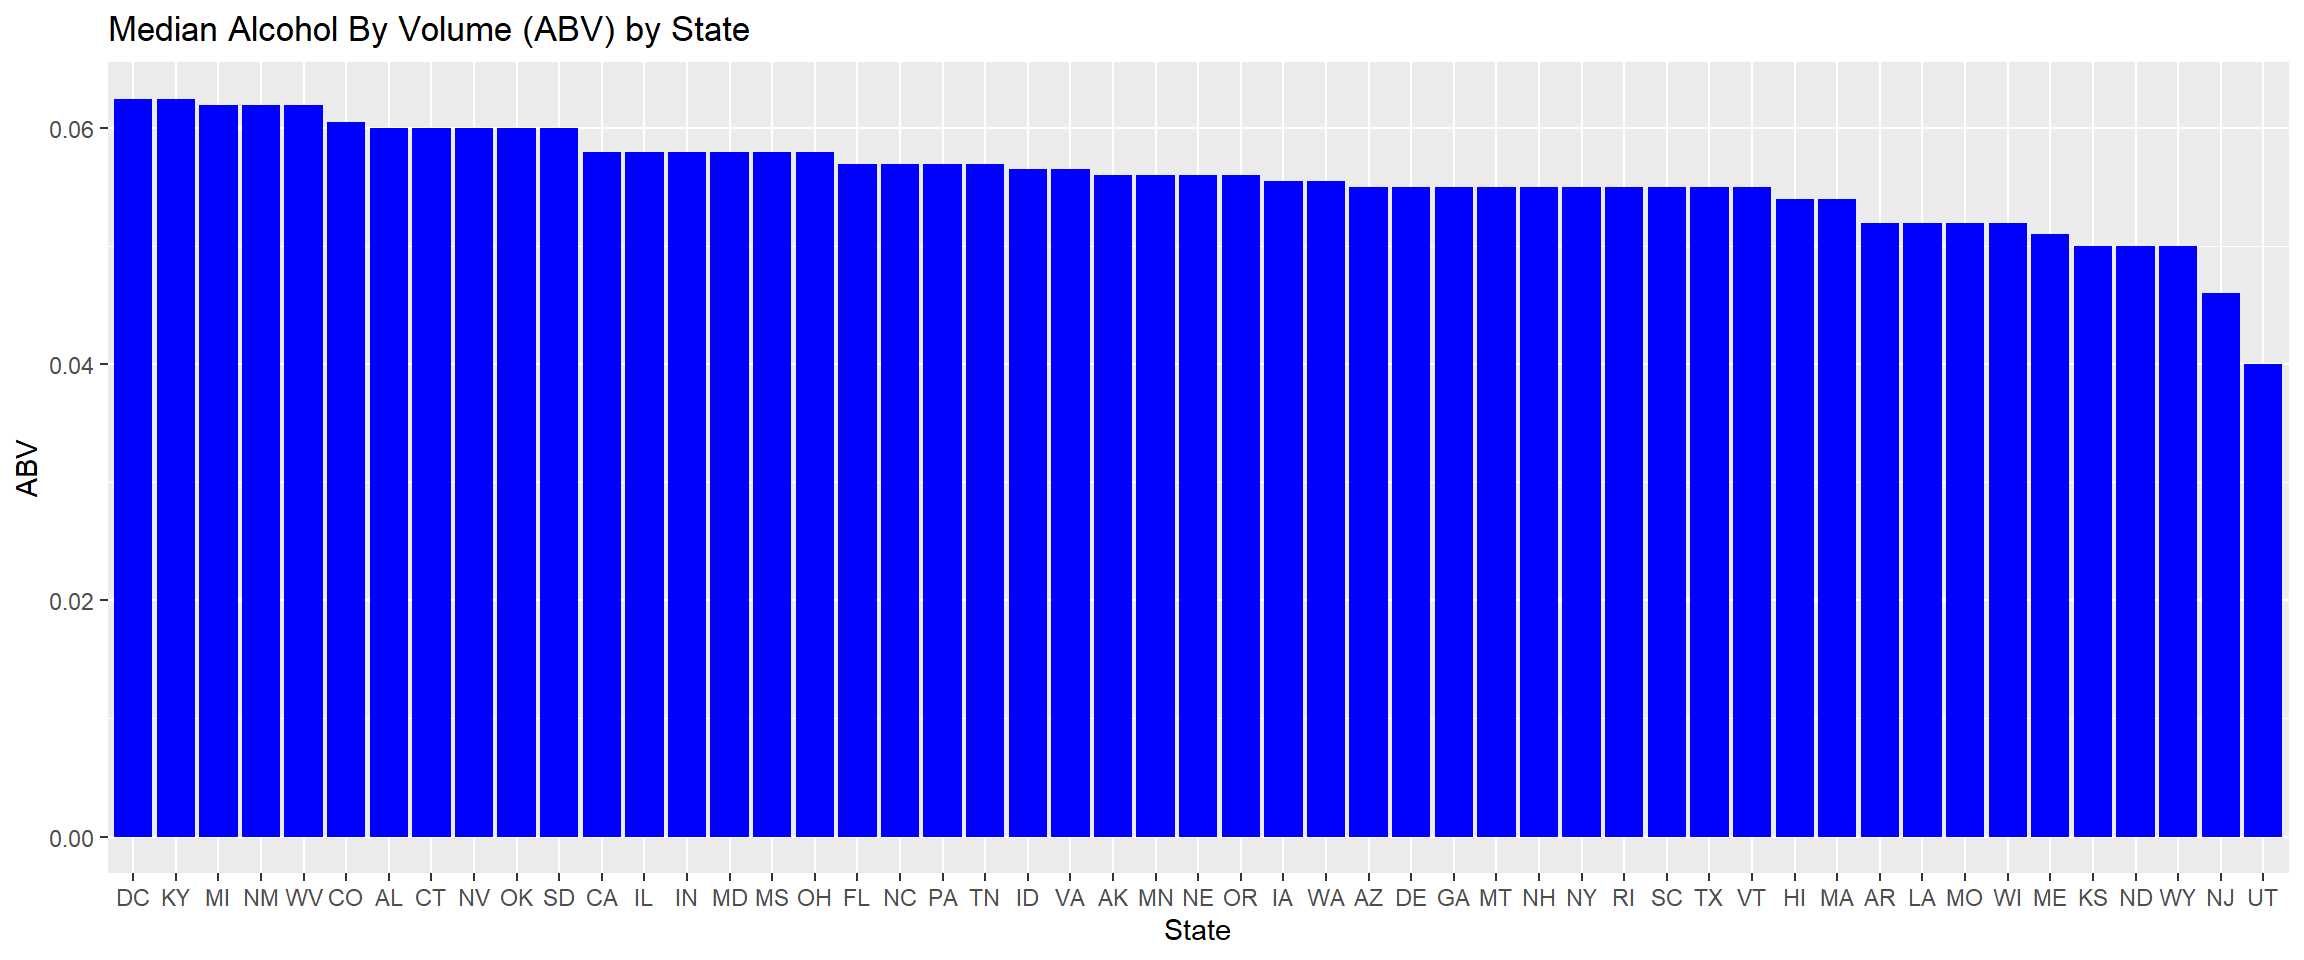
\includegraphics{Beer_Study_files/figure-latex/unnamed-chunk-7-1.pdf}

\begin{Shaded}
\begin{Highlighting}[]
\KeywordTok{ggplot}\NormalTok{(}\DataTypeTok{data=}\KeywordTok{aggregate}\NormalTok{(dfIBU}\OperatorTok{$}\NormalTok{IBU, }\DataTypeTok{by=}\KeywordTok{list}\NormalTok{(dfIBU}\OperatorTok{$}\NormalTok{State), }\DataTypeTok{FUN=}\NormalTok{median), }\DataTypeTok{mapping=}\KeywordTok{aes}\NormalTok{(}\DataTypeTok{x =} \KeywordTok{reorder}\NormalTok{(Group}\FloatTok{.1}\NormalTok{,}\OperatorTok{-}\NormalTok{x), }\DataTypeTok{y =}\NormalTok{ x)) }\OperatorTok{+}\StringTok{ }\KeywordTok{geom_bar}\NormalTok{(}\DataTypeTok{stat =} \StringTok{"identity"}\NormalTok{, }\DataTypeTok{fill=}\StringTok{"blue"}\NormalTok{) }\OperatorTok{+}\StringTok{ }\KeywordTok{xlab}\NormalTok{(}\StringTok{"State"}\NormalTok{) }\OperatorTok{+}\StringTok{ }\KeywordTok{ylab}\NormalTok{(}\StringTok{"IBU"}\NormalTok{) }\OperatorTok{+}\StringTok{ }\KeywordTok{ggtitle}\NormalTok{(}\StringTok{"Median International Bitterness Unit (IBU) by State"}\NormalTok{)}
\end{Highlighting}
\end{Shaded}

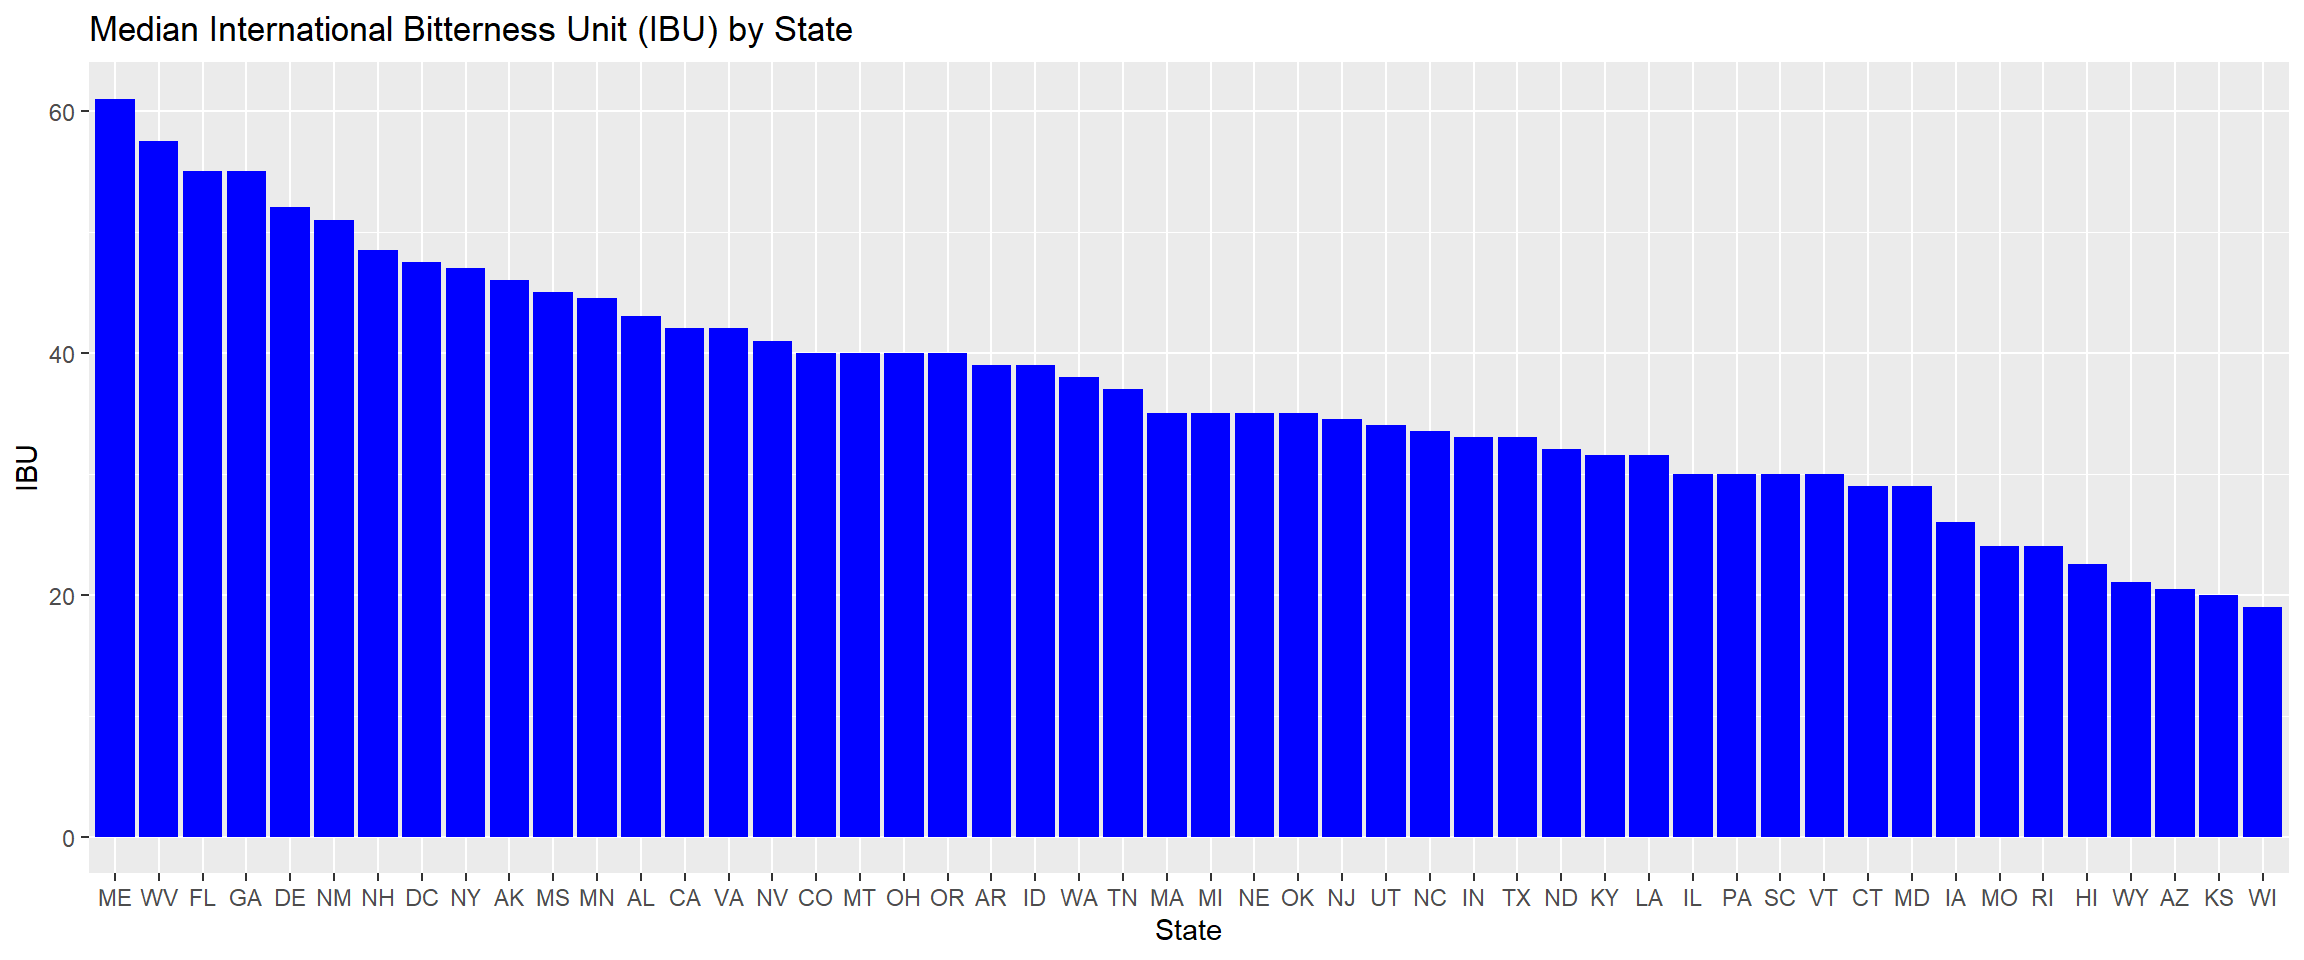
\includegraphics{Beer_Study_files/figure-latex/unnamed-chunk-7-2.pdf}

Generating map to look at Max Alcohol by Volume by State and Max IBU's
by State

\begin{Shaded}
\begin{Highlighting}[]
\KeywordTok{ggplot}\NormalTok{(}\DataTypeTok{data=}\KeywordTok{aggregate}\NormalTok{(dfABV}\OperatorTok{$}\NormalTok{ABV, }\DataTypeTok{by=}\KeywordTok{list}\NormalTok{(dfABV}\OperatorTok{$}\NormalTok{State), }\DataTypeTok{FUN=}\NormalTok{max), }\DataTypeTok{mapping=}\KeywordTok{aes}\NormalTok{(}\DataTypeTok{x =} \KeywordTok{reorder}\NormalTok{(Group}\FloatTok{.1}\NormalTok{,}\OperatorTok{-}\NormalTok{x), }\DataTypeTok{y =}\NormalTok{ x)) }\OperatorTok{+}\StringTok{ }\KeywordTok{geom_bar}\NormalTok{(}\DataTypeTok{stat =} \StringTok{"identity"}\NormalTok{, }\DataTypeTok{fill=}\StringTok{"blue"}\NormalTok{) }\OperatorTok{+}\StringTok{ }\KeywordTok{xlab}\NormalTok{(}\StringTok{"State"}\NormalTok{) }\OperatorTok{+}\StringTok{ }\KeywordTok{ylab}\NormalTok{(}\StringTok{"ABV"}\NormalTok{) }\OperatorTok{+}\StringTok{ }\KeywordTok{ggtitle}\NormalTok{(}\StringTok{"Maximum Alcohol By Volume (ABV) by State"}\NormalTok{)}
\end{Highlighting}
\end{Shaded}

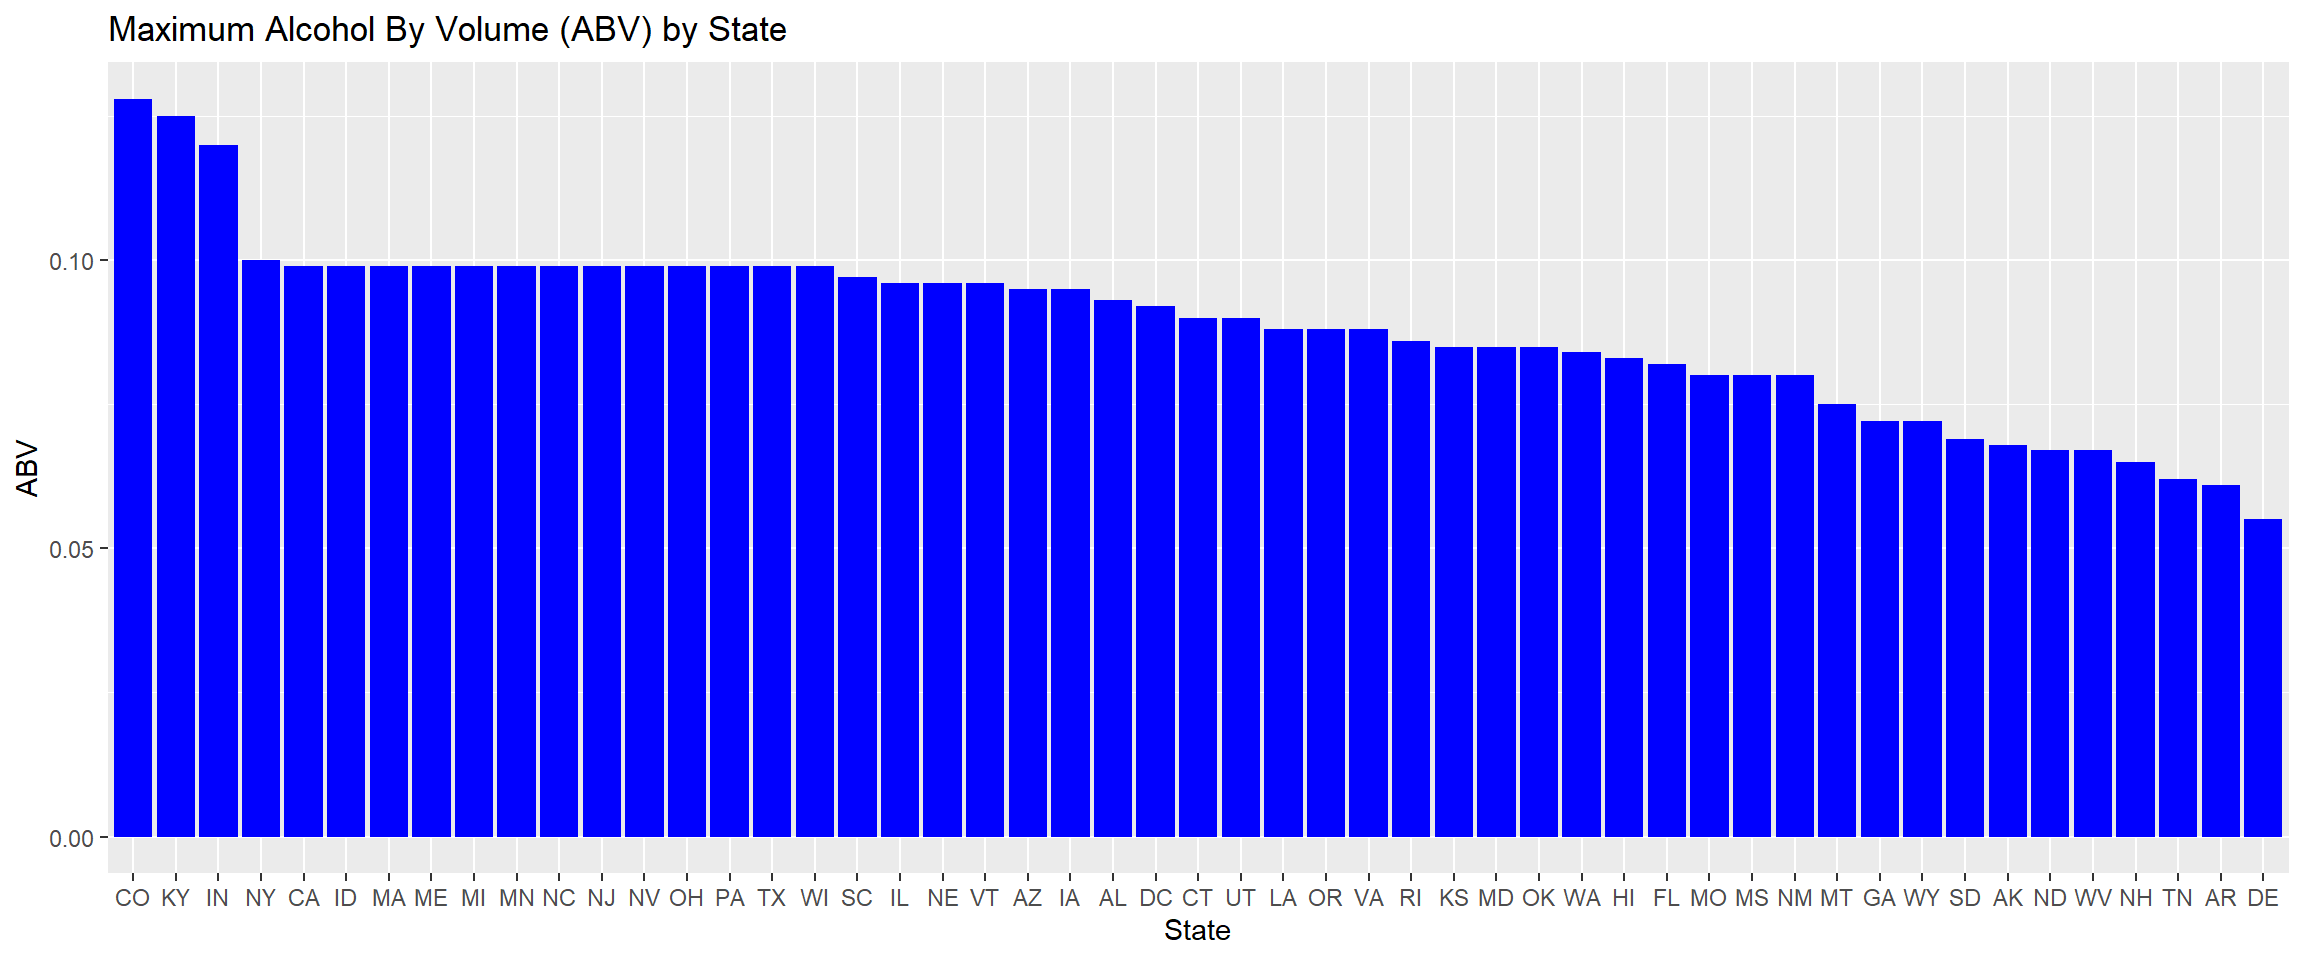
\includegraphics{Beer_Study_files/figure-latex/unnamed-chunk-8-1.pdf}

\begin{Shaded}
\begin{Highlighting}[]
\KeywordTok{ggplot}\NormalTok{(}\DataTypeTok{data=}\KeywordTok{aggregate}\NormalTok{(dfIBU}\OperatorTok{$}\NormalTok{IBU, }\DataTypeTok{by=}\KeywordTok{list}\NormalTok{(dfIBU}\OperatorTok{$}\NormalTok{State), }\DataTypeTok{FUN=}\NormalTok{max), }\DataTypeTok{mapping=}\KeywordTok{aes}\NormalTok{(}\DataTypeTok{x =} \KeywordTok{reorder}\NormalTok{(Group}\FloatTok{.1}\NormalTok{,}\OperatorTok{-}\NormalTok{x), }\DataTypeTok{y =}\NormalTok{ x)) }\OperatorTok{+}\StringTok{ }\KeywordTok{geom_bar}\NormalTok{(}\DataTypeTok{stat =} \StringTok{"identity"}\NormalTok{, }\DataTypeTok{fill=}\StringTok{"blue"}\NormalTok{) }\OperatorTok{+}\StringTok{ }\KeywordTok{xlab}\NormalTok{(}\StringTok{"State"}\NormalTok{) }\OperatorTok{+}\StringTok{ }\KeywordTok{ylab}\NormalTok{(}\StringTok{"IBU"}\NormalTok{) }\OperatorTok{+}\StringTok{ }\KeywordTok{ggtitle}\NormalTok{(}\StringTok{"Maximum International Bitterness Unit (IBU) by State"}\NormalTok{)}
\end{Highlighting}
\end{Shaded}

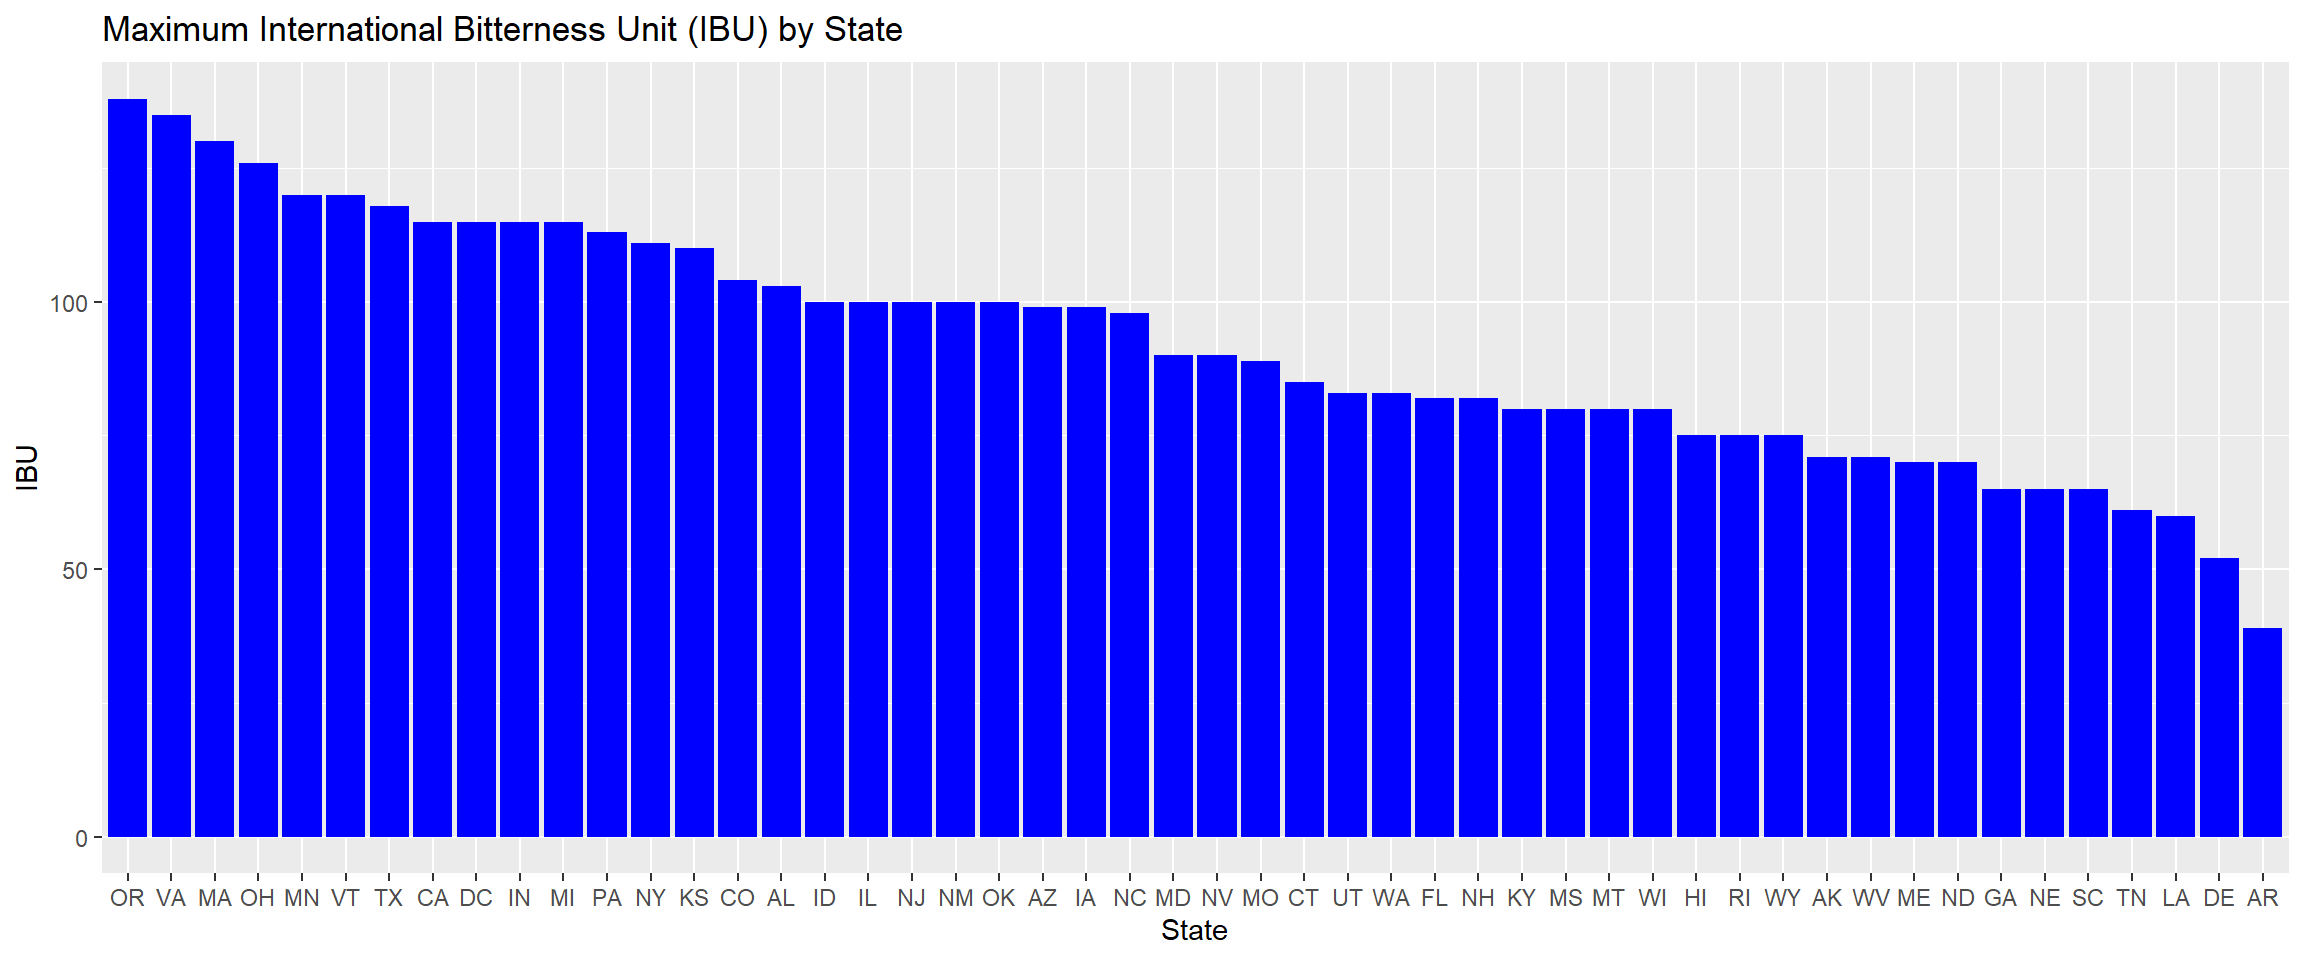
\includegraphics{Beer_Study_files/figure-latex/unnamed-chunk-8-2.pdf}

\begin{Shaded}
\begin{Highlighting}[]
\CommentTok{#Mapps of Max IBU by State }

\NormalTok{usa =}\StringTok{ }\KeywordTok{map_data}\NormalTok{(}\StringTok{"usa"}\NormalTok{)}

\NormalTok{p <-}\StringTok{ }\KeywordTok{ggplot}\NormalTok{() }\OperatorTok{+}\StringTok{ }
\StringTok{  }\KeywordTok{geom_polygon}\NormalTok{(}\DataTypeTok{data =}\NormalTok{ usa, }\KeywordTok{aes}\NormalTok{(}\DataTypeTok{x =}\NormalTok{ long, }\DataTypeTok{y =}\NormalTok{ lat, }\DataTypeTok{group =}\NormalTok{ group), }\DataTypeTok{fill =} \StringTok{"lightblue"}\NormalTok{, }\DataTypeTok{color =} \StringTok{"black"}\NormalTok{) }\OperatorTok{+}\StringTok{ }
\StringTok{  }\KeywordTok{coord_quickmap}\NormalTok{()}

\CommentTok{#takes aggregates and labels coordinates}

\NormalTok{agg =}\StringTok{ }\KeywordTok{aggregate}\NormalTok{(dfIBU}\OperatorTok{$}\NormalTok{IBU, }\DataTypeTok{by=}\KeywordTok{list}\NormalTok{(dfIBU}\OperatorTok{$}\NormalTok{State), }\DataTypeTok{FUN=}\NormalTok{max)}

\NormalTok{state_agg =}\StringTok{ }\KeywordTok{inner_join}\NormalTok{(agg, us_states, }\DataTypeTok{by =} \KeywordTok{c}\NormalTok{(}\StringTok{"Group.1"}\NormalTok{ =}\StringTok{ "state"}\NormalTok{))}

\NormalTok{state_agg =}\StringTok{ }\NormalTok{state_agg[}\KeywordTok{order}\NormalTok{(state_agg}\OperatorTok{$}\NormalTok{x, }\DataTypeTok{decreasing =} \OtherTok{TRUE}\NormalTok{)[}\DecValTok{1}\OperatorTok{:}\DecValTok{10}\NormalTok{],]}
  
\CommentTok{#layers on plots with each state and aggregate }


\NormalTok{p }\OperatorTok{+}\StringTok{ }\KeywordTok{geom_point}\NormalTok{(}\DataTypeTok{data =}\NormalTok{ state_agg, }\KeywordTok{aes}\NormalTok{(}\DataTypeTok{x =}\NormalTok{ longitude, }\DataTypeTok{y =}\NormalTok{ latitude)) }\OperatorTok{+}\StringTok{ }\KeywordTok{geom_text}\NormalTok{(}\DataTypeTok{data =}\NormalTok{ state_agg, }\KeywordTok{aes}\NormalTok{(}\DataTypeTok{x =}\NormalTok{ longitude, }\DataTypeTok{y =}\NormalTok{ latitude, }\DataTypeTok{label =}\NormalTok{ x), }\DataTypeTok{hjust =} \DecValTok{0}\NormalTok{ , }\DataTypeTok{nudge_x =} \FloatTok{0.75}\NormalTok{, }\DataTypeTok{color =} \StringTok{"red"}\NormalTok{ )}\OperatorTok{+}
\StringTok{   }\KeywordTok{geom_text}\NormalTok{(}\DataTypeTok{data =}\NormalTok{ state_agg, }\KeywordTok{aes}\NormalTok{(}\DataTypeTok{x =}\NormalTok{ longitude, }\DataTypeTok{y =}\NormalTok{ latitude, }\DataTypeTok{label =}\NormalTok{ name), }\DataTypeTok{hjust =} \DecValTok{1}\NormalTok{ , }\DataTypeTok{nudge_x =} \DecValTok{3}\NormalTok{, }\DataTypeTok{nudge_y =} \DecValTok{-1}\NormalTok{, }\DataTypeTok{color =} \StringTok{"red"}\NormalTok{ )}\OperatorTok{+}
\StringTok{  }\KeywordTok{coord_fixed}\NormalTok{(}\FloatTok{1.50}\NormalTok{) }\OperatorTok{+}\StringTok{ }\CommentTok{# fix lat/long display ratio}
\StringTok{  }\KeywordTok{ggtitle}\NormalTok{(}\StringTok{"Top 10 States with Greatest IBU"}\NormalTok{) }\OperatorTok{+}\StringTok{ }\KeywordTok{theme_bw}\NormalTok{() }\OperatorTok{+}\StringTok{ }\KeywordTok{theme}\NormalTok{(}\DataTypeTok{plot.title =} \KeywordTok{element_text}\NormalTok{(}\DataTypeTok{hjust =} \FloatTok{0.5}\NormalTok{)) }\OperatorTok{+}\StringTok{  }\KeywordTok{theme}\NormalTok{(}\DataTypeTok{panel.border =} \KeywordTok{element_blank}\NormalTok{(), }\DataTypeTok{panel.grid.major =} \KeywordTok{element_blank}\NormalTok{(), }\DataTypeTok{panel.grid.minor =} \KeywordTok{element_blank}\NormalTok{(), }\DataTypeTok{axis.line =} \KeywordTok{element_line}\NormalTok{(}\DataTypeTok{colour =} \StringTok{"Black"}\NormalTok{)) }\OperatorTok{+}\StringTok{ }
\StringTok{  }\KeywordTok{theme}\NormalTok{(}\DataTypeTok{legend.position =} \StringTok{"none"}\NormalTok{,}
        \DataTypeTok{axis.title.x=}\KeywordTok{element_blank}\NormalTok{(), }\CommentTok{# hide x axis title}
        \DataTypeTok{axis.text.x=}\KeywordTok{element_blank}\NormalTok{(),  }\CommentTok{# hide x axis text}
        \DataTypeTok{axis.ticks.x=}\KeywordTok{element_blank}\NormalTok{(), }\CommentTok{# hide x axis ticks}
        \DataTypeTok{axis.title.y=}\KeywordTok{element_blank}\NormalTok{(), }\CommentTok{# hide y axis title}
        \DataTypeTok{axis.text.y=}\KeywordTok{element_blank}\NormalTok{(),  }\CommentTok{# hide y axis text}
        \DataTypeTok{axis.ticks.y=}\KeywordTok{element_blank}\NormalTok{()) }\CommentTok{# hide y axis ticks}
\end{Highlighting}
\end{Shaded}

\begin{verbatim}
## Coordinate system already present. Adding new coordinate system, which will replace the existing one.
\end{verbatim}

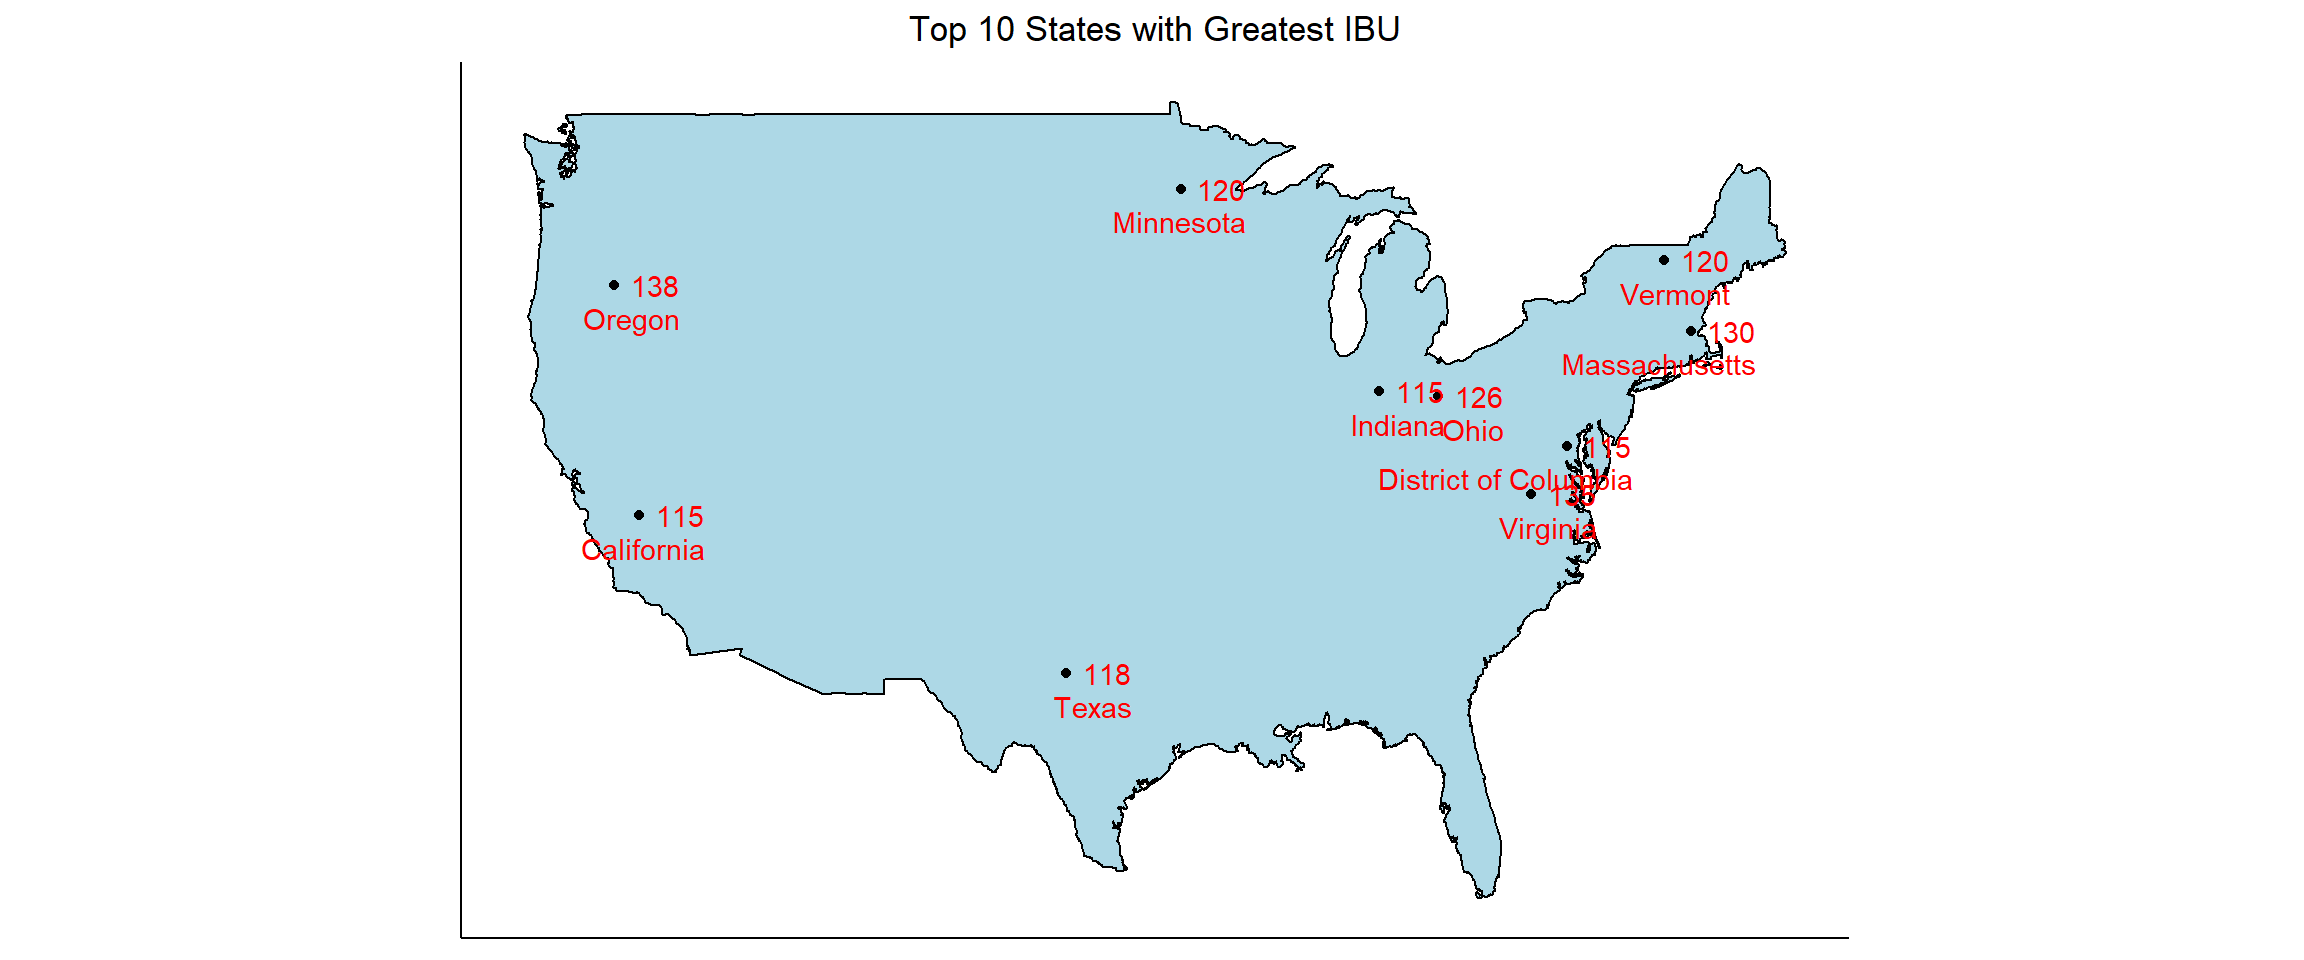
\includegraphics{Beer_Study_files/figure-latex/unnamed-chunk-8-3.pdf}

\begin{Shaded}
\begin{Highlighting}[]
\NormalTok{agg =}\StringTok{ }\KeywordTok{aggregate}\NormalTok{(dfABV}\OperatorTok{$}\NormalTok{ABV, }\DataTypeTok{by=}\KeywordTok{list}\NormalTok{(dfABV}\OperatorTok{$}\NormalTok{State), }\DataTypeTok{FUN=}\NormalTok{max)}

\NormalTok{state_agg =}\StringTok{ }\KeywordTok{inner_join}\NormalTok{(agg, us_states, }\DataTypeTok{by =} \KeywordTok{c}\NormalTok{(}\StringTok{"Group.1"}\NormalTok{ =}\StringTok{ "state"}\NormalTok{))}

\NormalTok{state_agg =}\StringTok{ }\NormalTok{state_agg[}\KeywordTok{order}\NormalTok{(state_agg}\OperatorTok{$}\NormalTok{x, }\DataTypeTok{decreasing =} \OtherTok{TRUE}\NormalTok{)[}\DecValTok{1}\OperatorTok{:}\DecValTok{10}\NormalTok{],]}


\NormalTok{p }\OperatorTok{+}\StringTok{ }\KeywordTok{geom_point}\NormalTok{(}\DataTypeTok{data =}\NormalTok{ state_agg, }\KeywordTok{aes}\NormalTok{(}\DataTypeTok{x =}\NormalTok{ longitude, }\DataTypeTok{y =}\NormalTok{ latitude)) }\OperatorTok{+}\StringTok{ }\KeywordTok{geom_text}\NormalTok{(}\DataTypeTok{data =}\NormalTok{ state_agg, }\KeywordTok{aes}\NormalTok{(}\DataTypeTok{x =}\NormalTok{ longitude, }\DataTypeTok{y =}\NormalTok{ latitude, }\DataTypeTok{label =} \KeywordTok{round}\NormalTok{((x}\OperatorTok{*}\DecValTok{100}\NormalTok{)), }\DataTypeTok{digits =} \DecValTok{3}\NormalTok{), }\DataTypeTok{hjust =} \DecValTok{0}\NormalTok{ , }\DataTypeTok{nudge_x =} \DecValTok{1}\NormalTok{, }\DataTypeTok{color =} \StringTok{"red"}\NormalTok{ )}\OperatorTok{+}
\StringTok{   }\KeywordTok{geom_text}\NormalTok{(}\DataTypeTok{data =}\NormalTok{ state_agg, }\KeywordTok{aes}\NormalTok{(}\DataTypeTok{x =}\NormalTok{ longitude, }\DataTypeTok{y =}\NormalTok{ latitude, }\DataTypeTok{label =}\NormalTok{ name), }\DataTypeTok{hjust =} \DecValTok{1}\NormalTok{ , }\DataTypeTok{nudge_x =} \DecValTok{2}\NormalTok{, }\DataTypeTok{nudge_y =} \DecValTok{-1}\NormalTok{, }\DataTypeTok{color =} \StringTok{"red"}\NormalTok{ )}\OperatorTok{+}
\StringTok{  }\KeywordTok{coord_fixed}\NormalTok{(}\FloatTok{1.50}\NormalTok{) }\OperatorTok{+}\StringTok{ }\CommentTok{# fix lat/long display ratio}
\StringTok{  }\KeywordTok{ggtitle}\NormalTok{(}\StringTok{"Top 10 States With Greatest ABV"}\NormalTok{) }\OperatorTok{+}\StringTok{ }\KeywordTok{theme_bw}\NormalTok{() }\OperatorTok{+}\StringTok{ }\KeywordTok{theme}\NormalTok{(}\DataTypeTok{plot.title =} \KeywordTok{element_text}\NormalTok{(}\DataTypeTok{hjust =} \FloatTok{0.5}\NormalTok{)) }\OperatorTok{+}\StringTok{  }\KeywordTok{theme}\NormalTok{(}\DataTypeTok{panel.border =} \KeywordTok{element_blank}\NormalTok{(), }\DataTypeTok{panel.grid.major =} \KeywordTok{element_blank}\NormalTok{(), }\DataTypeTok{panel.grid.minor =} \KeywordTok{element_blank}\NormalTok{(), }\DataTypeTok{axis.line =} \KeywordTok{element_line}\NormalTok{(}\DataTypeTok{colour =} \StringTok{"Black"}\NormalTok{)) }\OperatorTok{+}\StringTok{ }
\StringTok{  }\KeywordTok{theme}\NormalTok{(}\DataTypeTok{legend.position =} \StringTok{"none"}\NormalTok{,}
        \DataTypeTok{axis.title.x=}\KeywordTok{element_blank}\NormalTok{(), }\CommentTok{# hide x axis title}
        \DataTypeTok{axis.text.x=}\KeywordTok{element_blank}\NormalTok{(),  }\CommentTok{# hide x axis text}
        \DataTypeTok{axis.ticks.x=}\KeywordTok{element_blank}\NormalTok{(), }\CommentTok{# hide x axis ticks}
        \DataTypeTok{axis.title.y=}\KeywordTok{element_blank}\NormalTok{(), }\CommentTok{# hide y axis title}
        \DataTypeTok{axis.text.y=}\KeywordTok{element_blank}\NormalTok{(),  }\CommentTok{# hide y axis text}
        \DataTypeTok{axis.ticks.y=}\KeywordTok{element_blank}\NormalTok{()) }\CommentTok{# hide y axis ticks}
\end{Highlighting}
\end{Shaded}

\begin{verbatim}
## Warning: Ignoring unknown aesthetics: digits
\end{verbatim}

\begin{verbatim}
## Coordinate system already present. Adding new coordinate system, which will replace the existing one.
\end{verbatim}

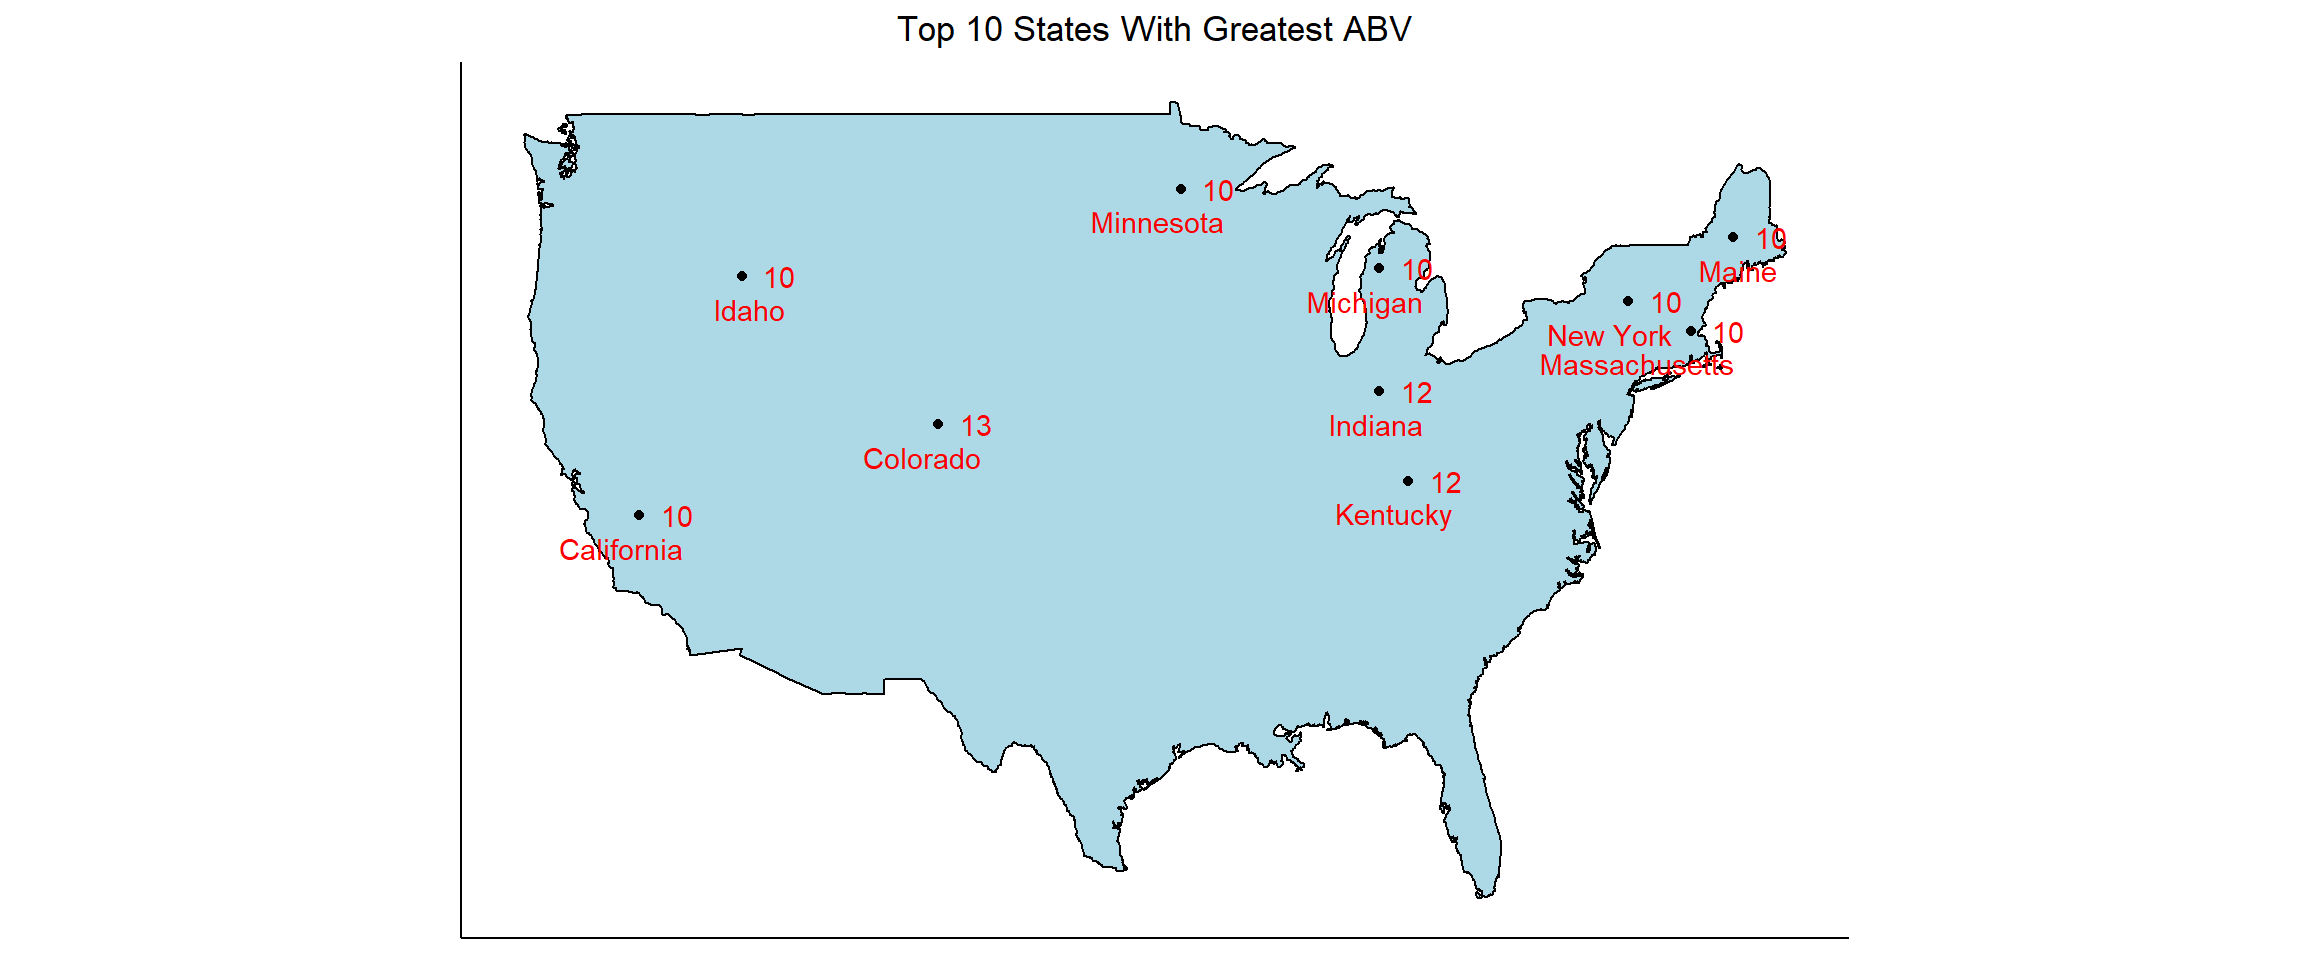
\includegraphics{Beer_Study_files/figure-latex/unnamed-chunk-8-4.pdf}
\textbf{Question of Interest: Comment on the Summary Statistics of ABV
and its Distribution}

\textbf{ABV Distribution + Summary Statistics}

\begin{Shaded}
\begin{Highlighting}[]
\KeywordTok{summary}\NormalTok{(dfABV}\OperatorTok{$}\NormalTok{ABV)}
\end{Highlighting}
\end{Shaded}

\begin{verbatim}
##    Min. 1st Qu.  Median    Mean 3rd Qu.    Max. 
## 0.00100 0.05000 0.05600 0.05977 0.06700 0.12800
\end{verbatim}

\textbf{Answer:} \textbf{We would like to get a better understanding of
the distribution of ABV to get a sense of what ABV most beers contain.
The majority of beers contain \textasciitilde.05 ABV}

\begin{Shaded}
\begin{Highlighting}[]
\KeywordTok{ggplot}\NormalTok{(dfABV, }\KeywordTok{aes}\NormalTok{(}\DataTypeTok{x=}\NormalTok{dfABV}\OperatorTok{$}\NormalTok{ABV)) }\OperatorTok{+}\StringTok{ }\KeywordTok{geom_histogram}\NormalTok{(}\DataTypeTok{colour=}\StringTok{"black"}\NormalTok{, }\DataTypeTok{fill=}\StringTok{"blue"}\NormalTok{) }\OperatorTok{+}\StringTok{ }\KeywordTok{xlab}\NormalTok{(}\StringTok{"ABV"}\NormalTok{) }\OperatorTok{+}\StringTok{ }\KeywordTok{ylab}\NormalTok{(}\StringTok{"Frequency"}\NormalTok{) }\OperatorTok{+}\StringTok{ }\KeywordTok{ggtitle}\NormalTok{(}\StringTok{"Distribution of ABV"}\NormalTok{)}
\end{Highlighting}
\end{Shaded}

\begin{verbatim}
## `stat_bin()` using `bins = 30`. Pick better value with `binwidth`.
\end{verbatim}

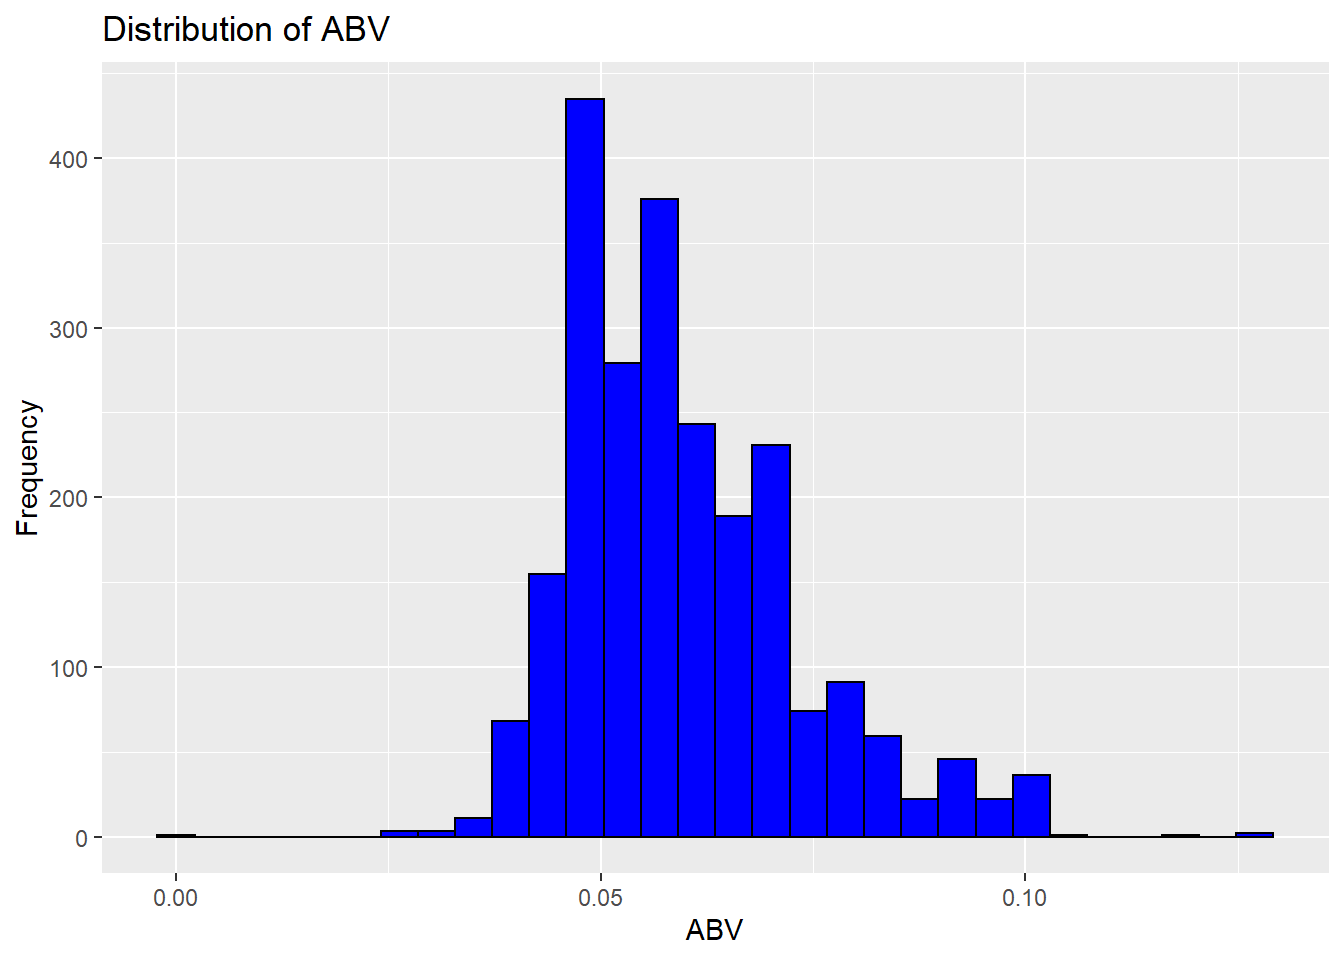
\includegraphics{Beer_Study_files/figure-latex/unnamed-chunk-10-1.pdf}

\begin{Shaded}
\begin{Highlighting}[]
\KeywordTok{ggplot}\NormalTok{(dfABV, }\KeywordTok{aes}\NormalTok{(}\DataTypeTok{x=}\NormalTok{dfABV}\OperatorTok{$}\NormalTok{Ales, }\DataTypeTok{y=}\NormalTok{dfABV}\OperatorTok{$}\NormalTok{ABV)) }\OperatorTok{+}\StringTok{ }\KeywordTok{geom_boxplot}\NormalTok{(}\DataTypeTok{outlier.color=}\StringTok{"black"}\NormalTok{, }\DataTypeTok{outlier.shape=}\DecValTok{16}\NormalTok{, }\DataTypeTok{outlier.size=}\DecValTok{2}\NormalTok{, }\DataTypeTok{notch=}\OtherTok{FALSE}\NormalTok{)}\OperatorTok{+}\StringTok{ }\KeywordTok{ggtitle}\NormalTok{(}\StringTok{"Boxplot of Ales vs ABV"}\NormalTok{)}\OperatorTok{+}\StringTok{ }\KeywordTok{xlab}\NormalTok{(}\StringTok{"Ales"}\NormalTok{) }\OperatorTok{+}\StringTok{ }\KeywordTok{ylab}\NormalTok{(}\StringTok{"ABV"}\NormalTok{)}
\end{Highlighting}
\end{Shaded}

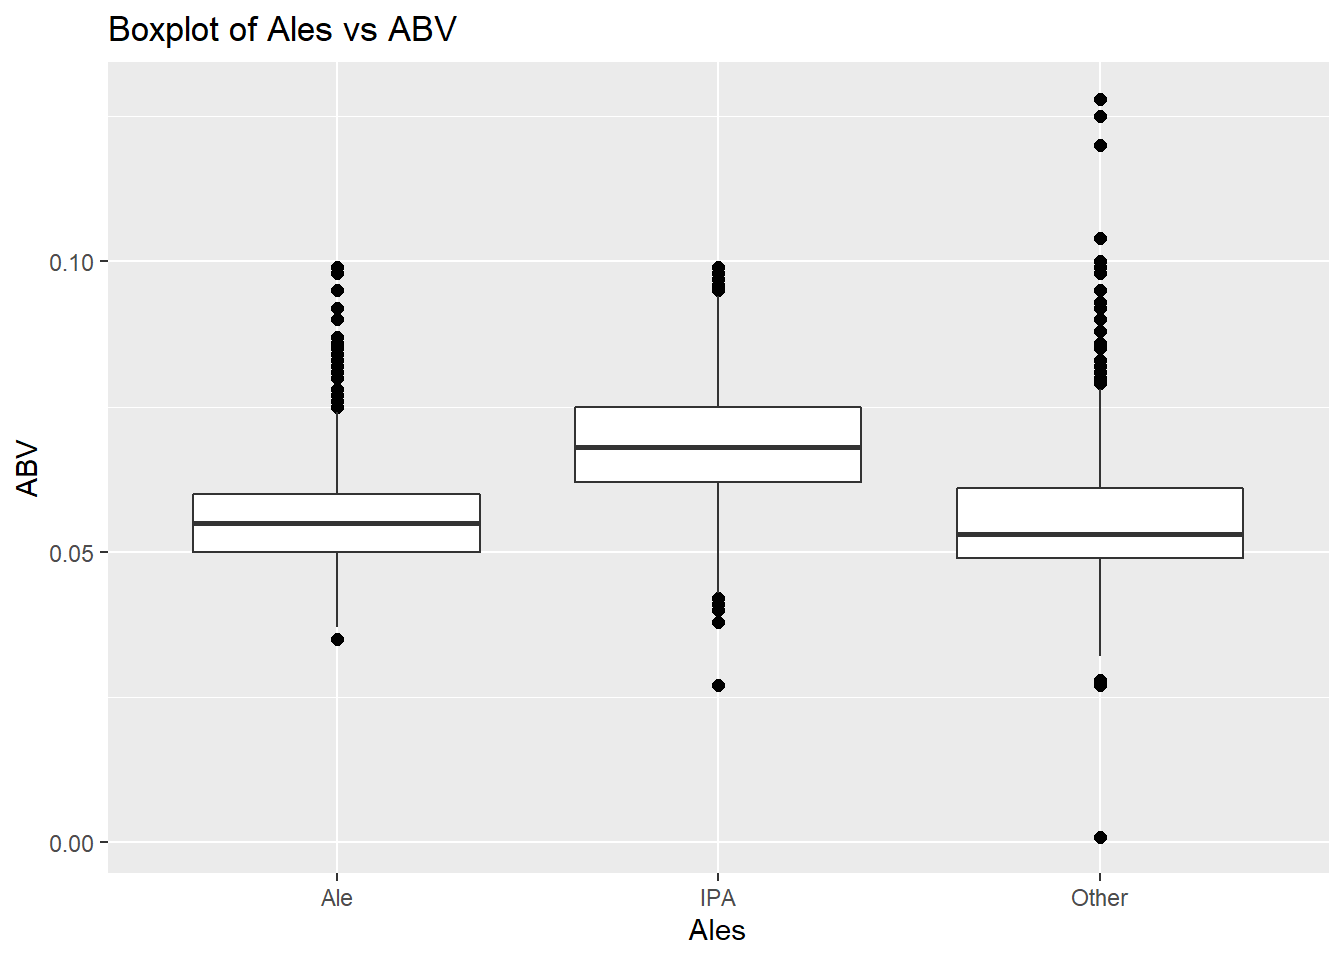
\includegraphics{Beer_Study_files/figure-latex/unnamed-chunk-10-2.pdf}

\textbf{Question of Interest: is there an apparent relationship between
the bitterness of the beer and its alcoholic content? Draw a scatter
plot. Make your best judgment of a relationship?}

\textbf{Answer:} \textbf{We would like to investigate whether there is a
relationship between ABV and IBU. To start out, we have created a
scatterplot of ABV to IBU to look for visual indication of a
relationship. We also checked by logging the variables to see if the
relationship observed increased. There does appear to be a slight
positive linear relationship, but we'll continue our analysis by
checking the correlation of these variables next.}

\begin{Shaded}
\begin{Highlighting}[]
\NormalTok{dfRM =}\StringTok{ }\KeywordTok{na.omit}\NormalTok{(dfFull)}
\NormalTok{dfRM[}\StringTok{"Log_IBU"}\NormalTok{] =}\StringTok{ }\KeywordTok{log}\NormalTok{(dfRM}\OperatorTok{$}\NormalTok{IBU)}
\NormalTok{dfRM[}\StringTok{"Log_ABV"}\NormalTok{] =}\StringTok{ }\KeywordTok{log}\NormalTok{(dfRM}\OperatorTok{$}\NormalTok{ABV)}
\NormalTok{dfRM[}\StringTok{"Logit_ABV"}\NormalTok{] =}\StringTok{ }\KeywordTok{logit}\NormalTok{(dfRM}\OperatorTok{$}\NormalTok{ABV)}
\KeywordTok{ggplot}\NormalTok{(}\DataTypeTok{data =}\NormalTok{ dfRM, }\DataTypeTok{mapping =} \KeywordTok{aes}\NormalTok{(}\DataTypeTok{x =}\NormalTok{ dfRM}\OperatorTok{$}\NormalTok{ABV, }\DataTypeTok{y =}\NormalTok{ dfRM}\OperatorTok{$}\NormalTok{IBU )) }\OperatorTok{+}\StringTok{ }\KeywordTok{geom_point}\NormalTok{() }\OperatorTok{+}\StringTok{ }\KeywordTok{xlab}\NormalTok{(}\StringTok{"ABV"}\NormalTok{) }\OperatorTok{+}\StringTok{ }\KeywordTok{ylab}\NormalTok{(}\StringTok{"IBU"}\NormalTok{) }\OperatorTok{+}\StringTok{ }\KeywordTok{ggtitle}\NormalTok{(}\StringTok{"Relatinship of ABV to IBU, ABV vs. IBU"}\NormalTok{)}
\end{Highlighting}
\end{Shaded}

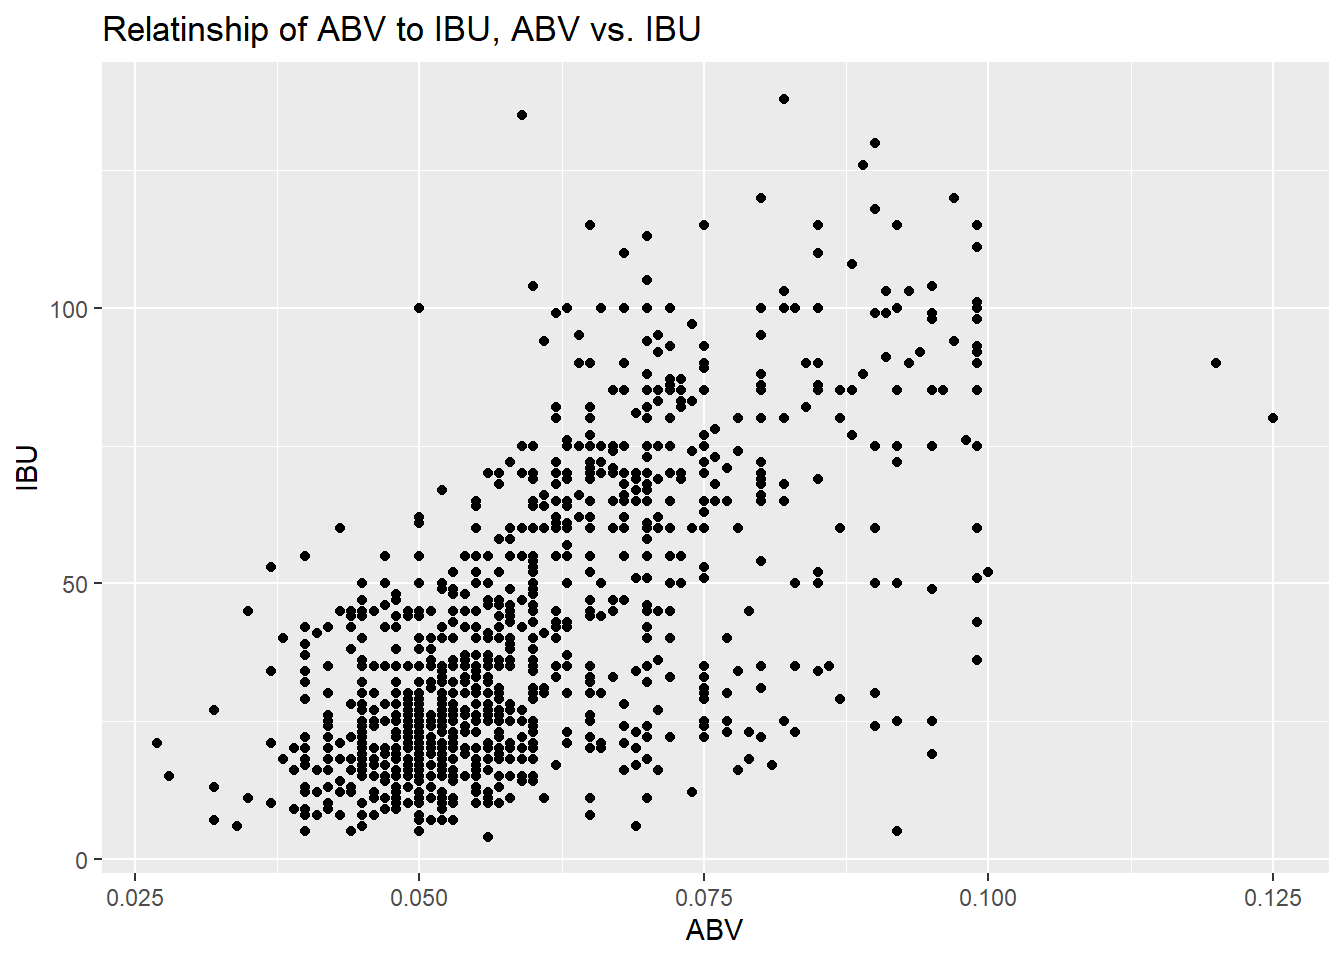
\includegraphics{Beer_Study_files/figure-latex/unnamed-chunk-11-1.pdf}

\begin{Shaded}
\begin{Highlighting}[]
\KeywordTok{ggplot}\NormalTok{(}\DataTypeTok{data =}\NormalTok{ dfRM, }\DataTypeTok{mapping =} \KeywordTok{aes}\NormalTok{(}\DataTypeTok{x =}\NormalTok{ dfRM}\OperatorTok{$}\NormalTok{Log_ABV, }\DataTypeTok{y =}\NormalTok{ dfRM}\OperatorTok{$}\NormalTok{Log_IBU )) }\OperatorTok{+}\StringTok{ }\KeywordTok{geom_point}\NormalTok{() }\OperatorTok{+}\StringTok{ }\KeywordTok{xlab}\NormalTok{(}\StringTok{"Log_ABV"}\NormalTok{) }\OperatorTok{+}\StringTok{ }\KeywordTok{ylab}\NormalTok{(}\StringTok{"Log_IBU"}\NormalTok{) }\OperatorTok{+}\StringTok{ }\KeywordTok{ggtitle}\NormalTok{(}\StringTok{"Relatinship of ABV to IBU, Log ABV vs. Log IBU"}\NormalTok{) }\OperatorTok{+}\StringTok{ }\KeywordTok{geom_smooth}\NormalTok{()}
\end{Highlighting}
\end{Shaded}

\begin{verbatim}
## `geom_smooth()` using method = 'gam' and formula 'y ~ s(x, bs = "cs")'
\end{verbatim}

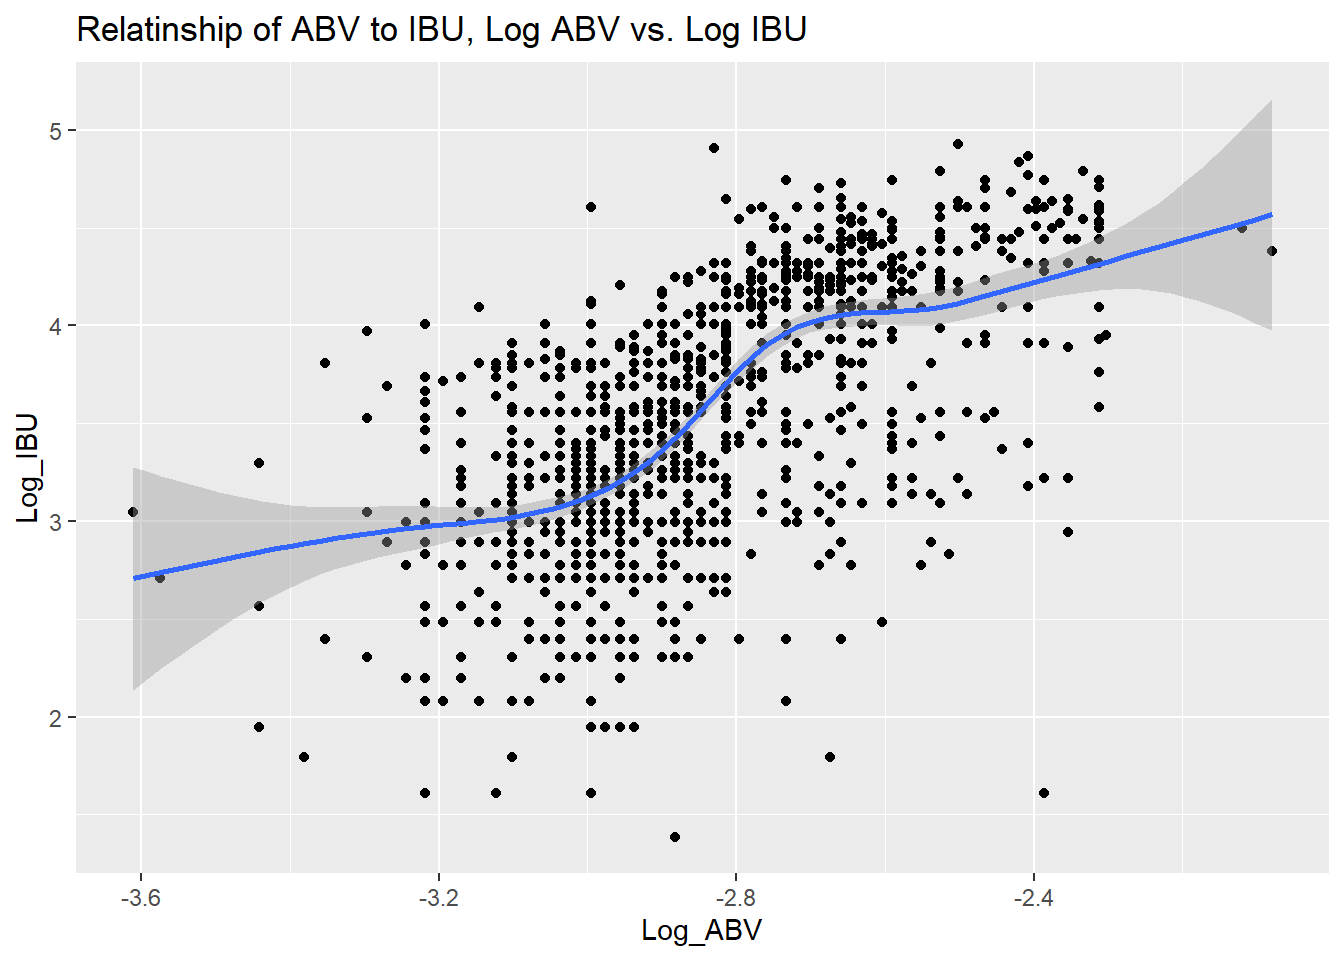
\includegraphics{Beer_Study_files/figure-latex/unnamed-chunk-11-2.pdf}

\begin{Shaded}
\begin{Highlighting}[]
\KeywordTok{ggplot}\NormalTok{(}\DataTypeTok{data =}\NormalTok{ dfRM, }\DataTypeTok{mapping =} \KeywordTok{aes}\NormalTok{(}\DataTypeTok{x =}\NormalTok{ dfRM}\OperatorTok{$}\NormalTok{Logit_ABV, }\DataTypeTok{y =}\NormalTok{ dfRM}\OperatorTok{$}\NormalTok{IBU )) }\OperatorTok{+}\StringTok{ }\KeywordTok{geom_point}\NormalTok{() }\OperatorTok{+}\StringTok{ }\KeywordTok{xlab}\NormalTok{(}\StringTok{"Logit_ABV"}\NormalTok{) }\OperatorTok{+}\StringTok{ }\KeywordTok{ylab}\NormalTok{(}\StringTok{"IBU"}\NormalTok{) }\OperatorTok{+}\StringTok{ }\KeywordTok{ggtitle}\NormalTok{(}\StringTok{"Relationship of ABV to IBU, Logit ABV vs. IBU"}\NormalTok{) }\OperatorTok{+}\StringTok{ }\KeywordTok{geom_smooth}\NormalTok{()}
\end{Highlighting}
\end{Shaded}

\begin{verbatim}
## `geom_smooth()` using method = 'gam' and formula 'y ~ s(x, bs = "cs")'
\end{verbatim}

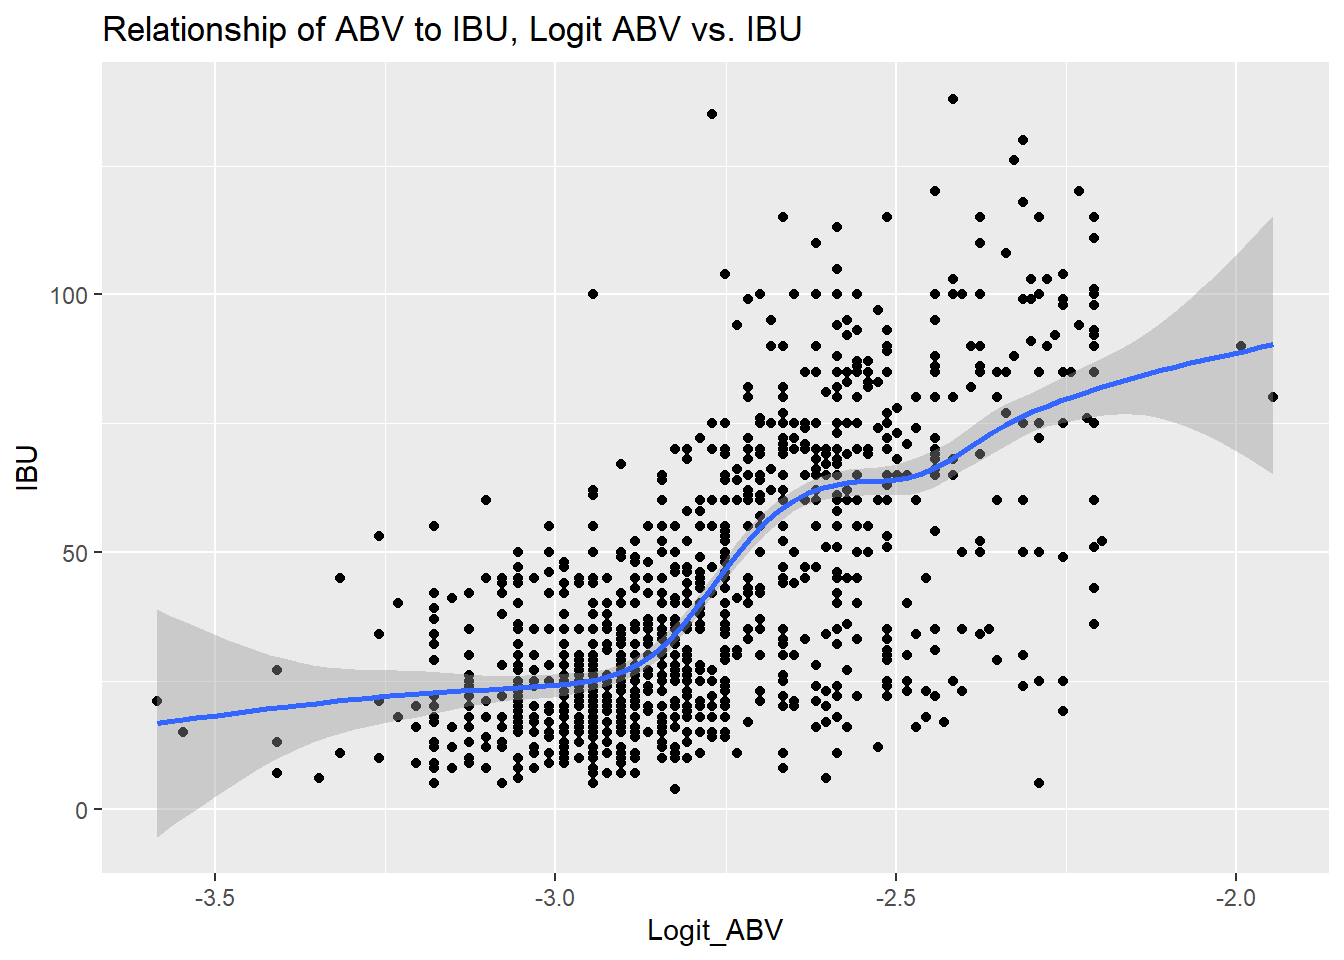
\includegraphics{Beer_Study_files/figure-latex/unnamed-chunk-11-3.pdf}

\begin{Shaded}
\begin{Highlighting}[]
\KeywordTok{ggplot}\NormalTok{(}\DataTypeTok{data =}\NormalTok{ dfRM, }\DataTypeTok{mapping =} \KeywordTok{aes}\NormalTok{(}\DataTypeTok{x =}\NormalTok{ dfRM}\OperatorTok{$}\NormalTok{Logit_ABV, }\DataTypeTok{y =}\NormalTok{ dfRM}\OperatorTok{$}\NormalTok{Log_IBU, }\DataTypeTok{color =}\NormalTok{ Ales)) }\OperatorTok{+}\StringTok{ }\KeywordTok{geom_point}\NormalTok{() }\OperatorTok{+}\StringTok{ }\KeywordTok{xlab}\NormalTok{(}\StringTok{"Logit_ABV"}\NormalTok{) }\OperatorTok{+}\StringTok{ }\KeywordTok{ylab}\NormalTok{(}\StringTok{"Log_IBU"}\NormalTok{) }\OperatorTok{+}\StringTok{ }\KeywordTok{ggtitle}\NormalTok{(}\StringTok{"Relationship of ABV to IBU, Logit ABV vs. Log IBU"}\NormalTok{)}
\end{Highlighting}
\end{Shaded}

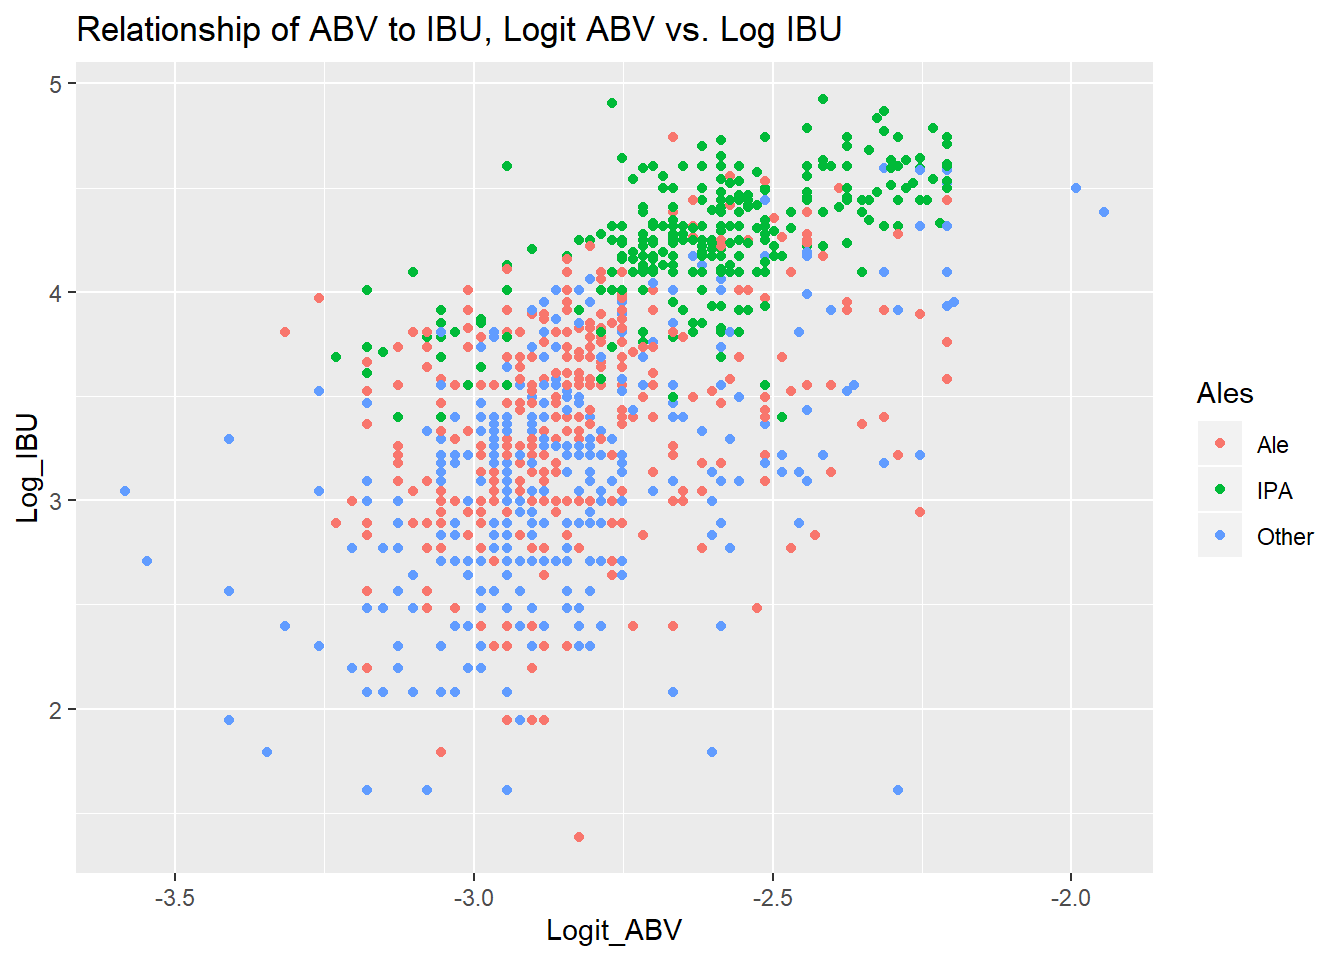
\includegraphics{Beer_Study_files/figure-latex/unnamed-chunk-11-4.pdf}

\begin{Shaded}
\begin{Highlighting}[]
\KeywordTok{ggplot}\NormalTok{(}\DataTypeTok{data =}\NormalTok{ dfRM, }\DataTypeTok{mapping =} \KeywordTok{aes}\NormalTok{(}\DataTypeTok{x =}\NormalTok{ dfRM}\OperatorTok{$}\NormalTok{Logit_ABV, }\DataTypeTok{y =}\NormalTok{ dfRM}\OperatorTok{$}\NormalTok{Log_IBU)) }\OperatorTok{+}\StringTok{ }\KeywordTok{geom_point}\NormalTok{() }\OperatorTok{+}\StringTok{ }\KeywordTok{xlab}\NormalTok{(}\StringTok{"Logit_ABV"}\NormalTok{) }\OperatorTok{+}\StringTok{ }\KeywordTok{ylab}\NormalTok{(}\StringTok{"Log_IBU"}\NormalTok{) }\OperatorTok{+}\StringTok{ }\KeywordTok{ggtitle}\NormalTok{(}\StringTok{"Relationship of ABV to IBU, Logit ABV vs. Log IBU"}\NormalTok{) }\OperatorTok{+}\StringTok{ }\KeywordTok{geom_smooth}\NormalTok{()}
\end{Highlighting}
\end{Shaded}

\begin{verbatim}
## `geom_smooth()` using method = 'gam' and formula 'y ~ s(x, bs = "cs")'
\end{verbatim}

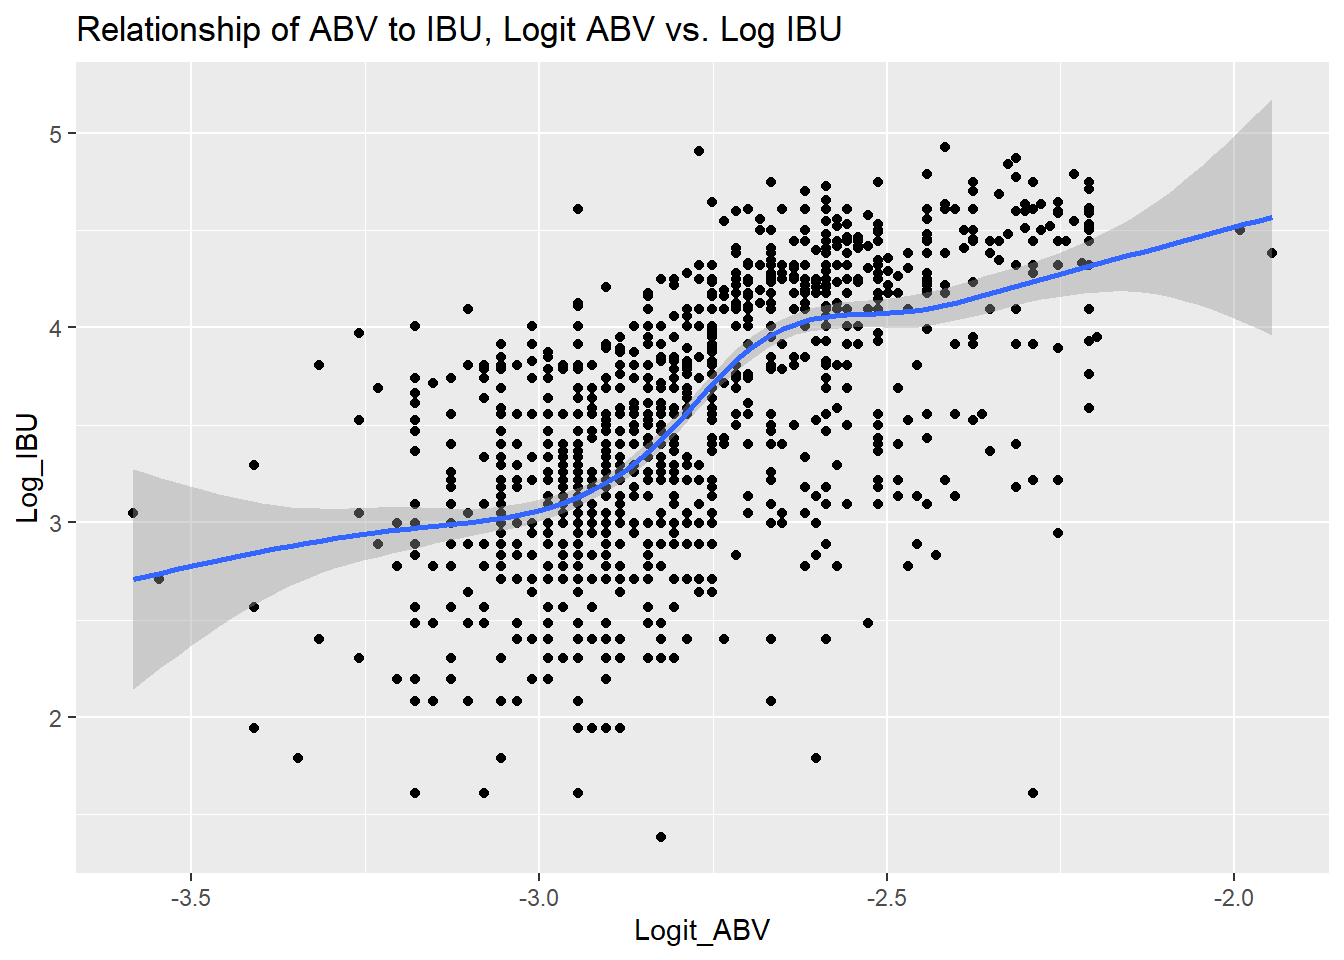
\includegraphics{Beer_Study_files/figure-latex/unnamed-chunk-11-5.pdf}

\textbf{Question of Interest: Is there an apparent relationship between
the bitterness of the beer and its alcoholic content? }

\textbf{Answer:}

\textbf{We would like to investigate if there is a relationship between
the bitterness of the beer and it's alcoholic content while at the same
time trying to identify a relationship between Ales, IPA's and other
styles of beer. Looking at the relationship of ABV and IBU to Ales, IPA
and other style of beer we can see there is a positive correlation
between ABV and IBU and we can also see evidence of clusters around the
styles of beer. To do this in a more formal manner, we perform a pearson
correlation between the two variables. The result is a positive
correlation with a pearsons correlation value of 0.671.}

\begin{Shaded}
\begin{Highlighting}[]
\KeywordTok{library}\NormalTok{(GGally)}
\NormalTok{dfRM }\OperatorTok\StringTok{ }
\KeywordTok{select}\NormalTok{(ABV, IBU) }\OperatorTok\StringTok{ }
\KeywordTok{ggpairs}\NormalTok{(}\DataTypeTok{title =} \StringTok{"ABV vs. IBU"}\NormalTok{)}
\end{Highlighting}
\end{Shaded}

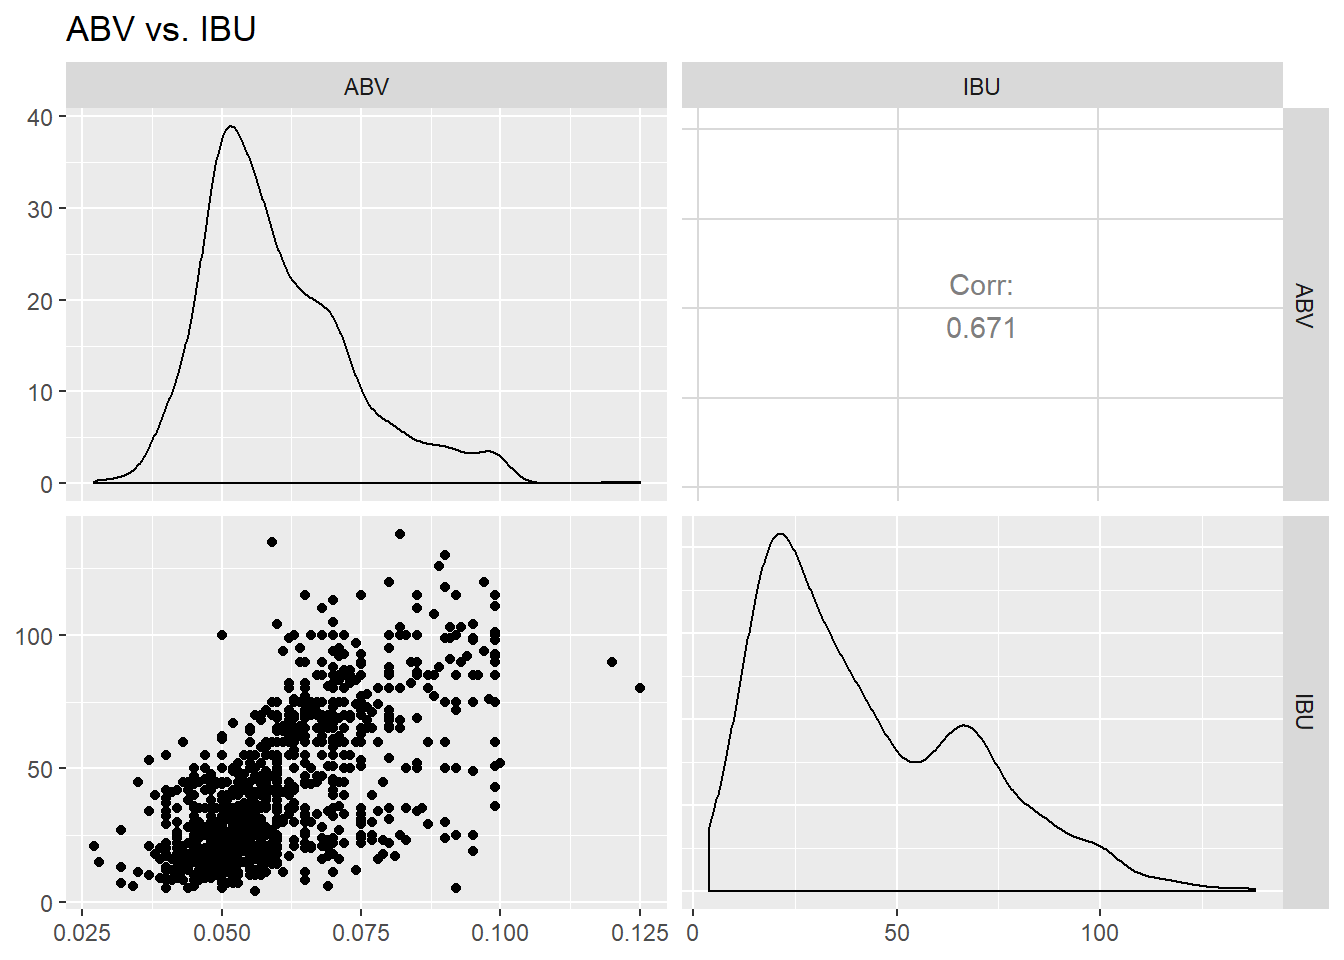
\includegraphics{Beer_Study_files/figure-latex/unnamed-chunk-12-1.pdf}

\begin{Shaded}
\begin{Highlighting}[]
\NormalTok{dfRM }\OperatorTok\StringTok{ }\KeywordTok{select}\NormalTok{(Logit_ABV, Log_IBU) }\OperatorTok\StringTok{ }\KeywordTok{ggpairs}\NormalTok{(}\DataTypeTok{title =} \StringTok{"Logit_ABV vs. Log_IBU"}\NormalTok{)}
\end{Highlighting}
\end{Shaded}

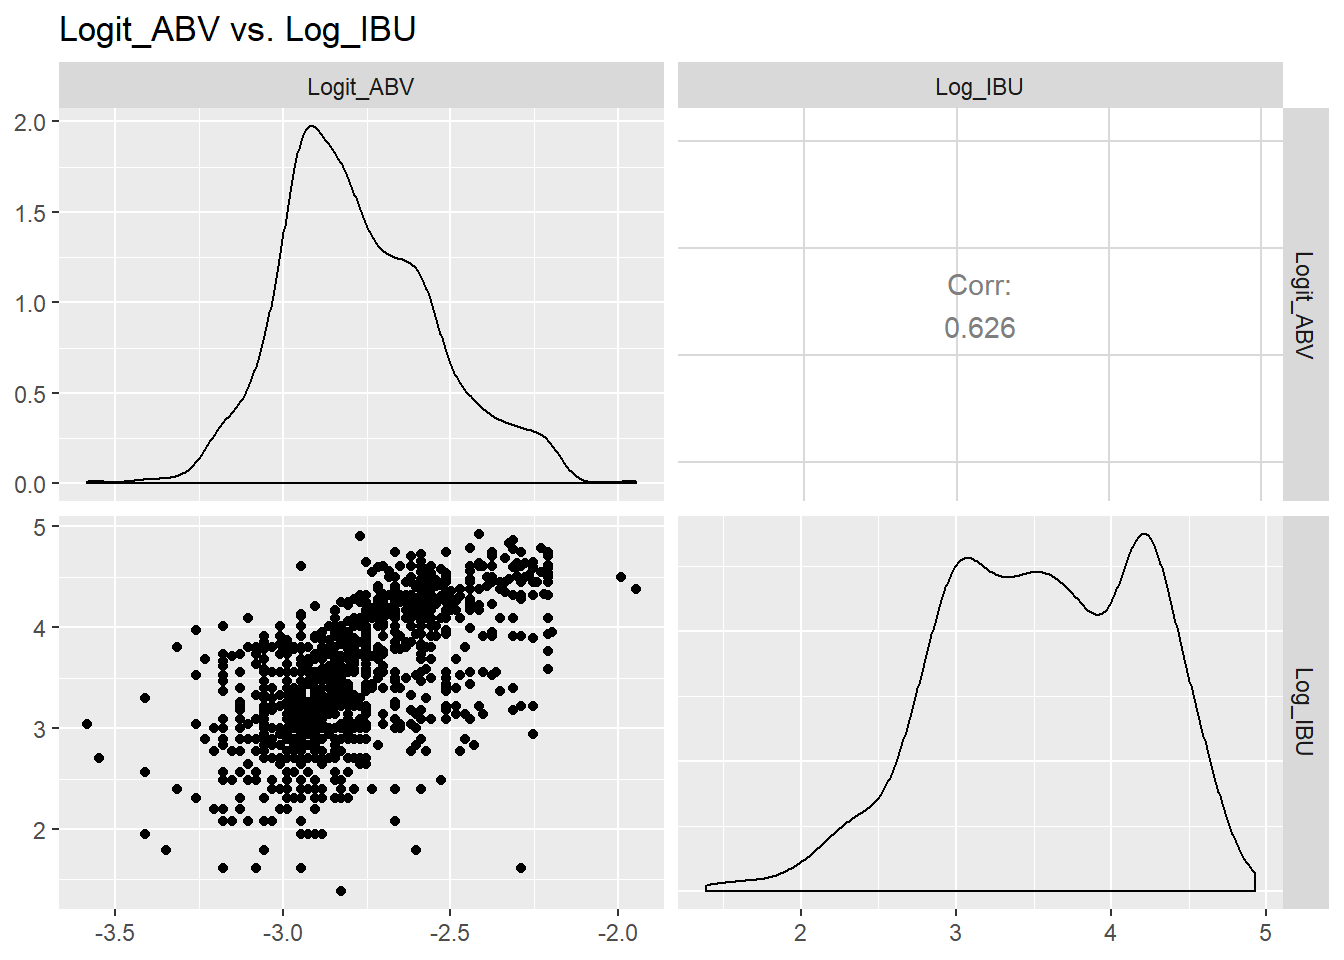
\includegraphics{Beer_Study_files/figure-latex/unnamed-chunk-12-2.pdf}

\begin{Shaded}
\begin{Highlighting}[]
\NormalTok{dfRM }\OperatorTok\StringTok{ }
\KeywordTok{select}\NormalTok{(ABV, IBU, Ales) }\OperatorTok\StringTok{ }
\KeywordTok{ggpairs}\NormalTok{(}\KeywordTok{aes}\NormalTok{(}\DataTypeTok{color =}\NormalTok{ Ales))}
\end{Highlighting}
\end{Shaded}

\begin{verbatim}
## `stat_bin()` using `bins = 30`. Pick better value with `binwidth`.
## `stat_bin()` using `bins = 30`. Pick better value with `binwidth`.
\end{verbatim}

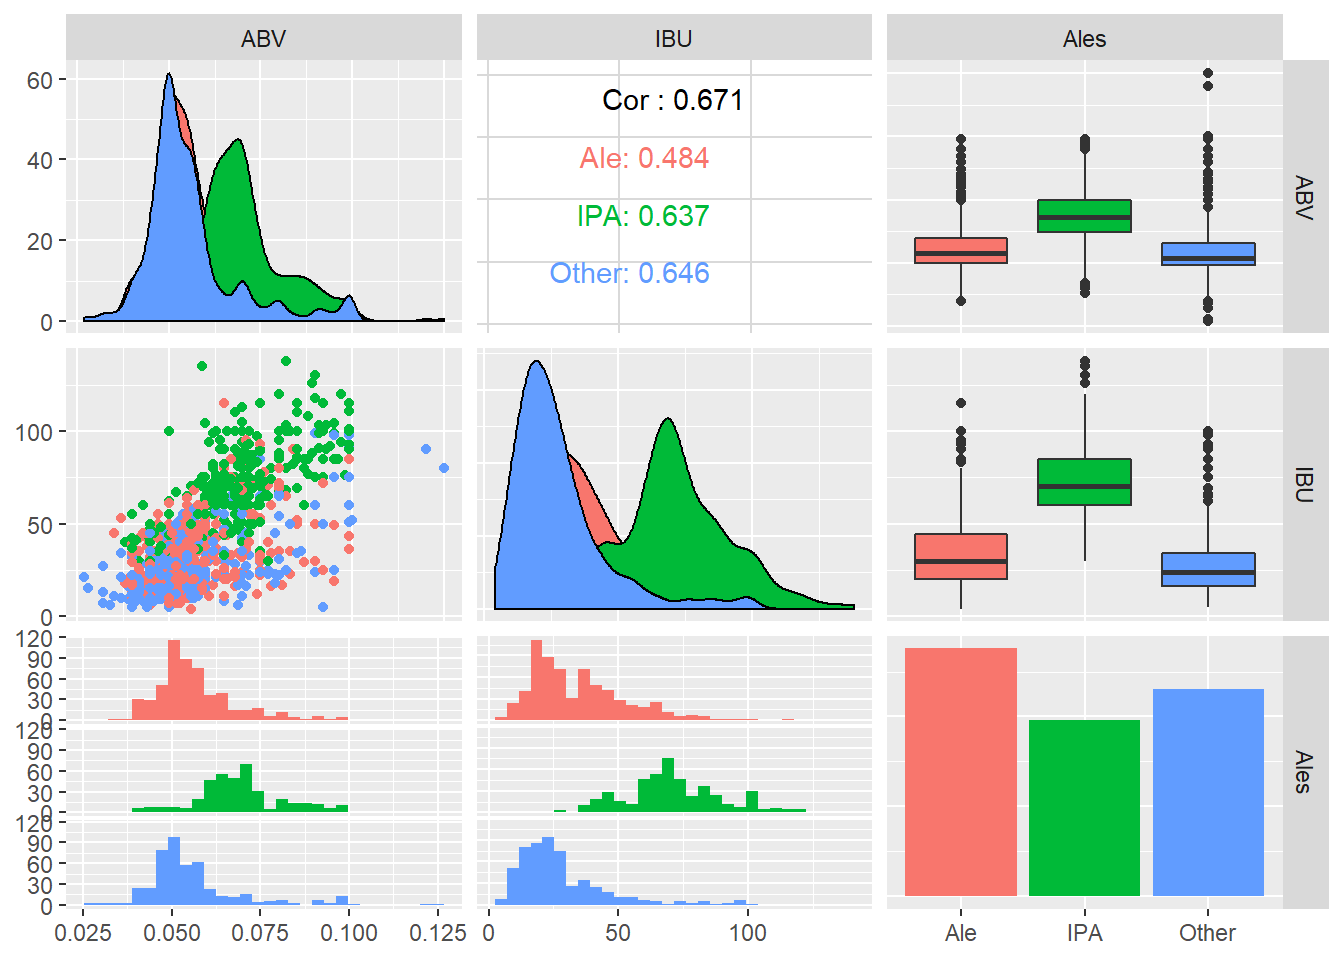
\includegraphics{Beer_Study_files/figure-latex/unnamed-chunk-13-1.pdf}

\begin{Shaded}
\begin{Highlighting}[]
\CommentTok{#Adding output from Pearson's product moment correlation test}

\KeywordTok{cor.test}\NormalTok{(dfRM}\OperatorTok{$}\NormalTok{ABV, dfRM}\OperatorTok{$}\NormalTok{IBU, }\DataTypeTok{method=}\KeywordTok{c}\NormalTok{(}\StringTok{"pearson"}\NormalTok{, }\StringTok{"kendall"}\NormalTok{, }\StringTok{"spearman"}\NormalTok{))}
\end{Highlighting}
\end{Shaded}

\begin{verbatim}
## 
##  Pearson's product-moment correlation
## 
## data:  dfRM$ABV and dfRM$IBU
## t = 33.863, df = 1403, p-value < 2.2e-16
## alternative hypothesis: true correlation is not equal to 0
## 95 percent confidence interval:
##  0.6407982 0.6984238
## sample estimates:
##       cor 
## 0.6706215
\end{verbatim}

\textbf{Question of Interest: Is there a difference with respect to IBU
and ABV between IPAs (India Pale Ales) and other types of Ale (any beer
with ``Ale'' in its name other than IPA)?}

\textbf{Answer:}

\textbf{We would like to investigate the difference with respect to IBU
and ABV between IPAs and other types of Ale. To do this, we will
construct both a KNN (k- Nearest Neighbor) model and NBB (Nieve-Bayes)we
construct a dataframe to include only the ABV, IBU and Ales indicator,
excluding missing values, to build a training and test set for further
analysis.}

\begin{Shaded}
\begin{Highlighting}[]
\KeywordTok{library}\NormalTok{(dplyr)}

\KeywordTok{set.seed}\NormalTok{(}\DecValTok{6}\NormalTok{)}
\NormalTok{splitPerc =}\StringTok{ }\FloatTok{.75}

\NormalTok{dfAles =}\StringTok{ }\NormalTok{dfRM }\OperatorTok\StringTok{ }\KeywordTok{filter}\NormalTok{(Ales }\OperatorTok{==}\StringTok{ "Ale"} \OperatorTok{|}\StringTok{ }\NormalTok{Ales }\OperatorTok{==}\StringTok{ "IPA"}\NormalTok{)}
\NormalTok{dfAles =}\StringTok{ }\NormalTok{dfAles }\OperatorTok\StringTok{ }\KeywordTok{select}\NormalTok{(ABV,IBU,Ales)}
\KeywordTok{summary}\NormalTok{(dfAles)}
\end{Highlighting}
\end{Shaded}

\begin{verbatim}
##       ABV               IBU            Ales    
##  Min.   :0.03500   Min.   :  4.00   Ale  :552  
##  1st Qu.:0.05200   1st Qu.: 27.00   IPA  :392  
##  Median :0.06000   Median : 45.00   Other:  0  
##  Mean   :0.06178   Mean   : 49.95              
##  3rd Qu.:0.07000   3rd Qu.: 70.00              
##  Max.   :0.09900   Max.   :138.00
\end{verbatim}

\begin{Shaded}
\begin{Highlighting}[]
\NormalTok{dfAles =}\StringTok{ }\KeywordTok{droplevels}\NormalTok{(dfAles,}\DataTypeTok{exclude =} \StringTok{"Other"}\NormalTok{)}
\KeywordTok{summary}\NormalTok{(dfAles)}
\end{Highlighting}
\end{Shaded}

\begin{verbatim}
##       ABV               IBU          Ales    
##  Min.   :0.03500   Min.   :  4.00   Ale:552  
##  1st Qu.:0.05200   1st Qu.: 27.00   IPA:392  
##  Median :0.06000   Median : 45.00            
##  Mean   :0.06178   Mean   : 49.95            
##  3rd Qu.:0.07000   3rd Qu.: 70.00            
##  Max.   :0.09900   Max.   :138.00
\end{verbatim}

\begin{Shaded}
\begin{Highlighting}[]
\NormalTok{trainIndices =}\StringTok{ }\KeywordTok{sample}\NormalTok{(}\DecValTok{1}\OperatorTok{:}\KeywordTok{dim}\NormalTok{(dfAles)[}\DecValTok{1}\NormalTok{],}\KeywordTok{round}\NormalTok{(splitPerc }\OperatorTok{*}\StringTok{ }\KeywordTok{dim}\NormalTok{(dfAles)[}\DecValTok{1}\NormalTok{]))}
\NormalTok{train =}\StringTok{ }\NormalTok{dfAles[trainIndices,]}
\NormalTok{test =}\StringTok{ }\NormalTok{dfAles[}\OperatorTok{-}\NormalTok{trainIndices,]}
\KeywordTok{colnames}\NormalTok{(dfAles)[}\KeywordTok{colSums}\NormalTok{(}\KeywordTok{is.na}\NormalTok{(dfAles))}\OperatorTok{>}\DecValTok{0}\NormalTok{]}
\end{Highlighting}
\end{Shaded}

\begin{verbatim}
## character(0)
\end{verbatim}

\textbf{Next, we want to iterate through multiple classification
attempts where we test with k=1 to 30 to determine the optimal k value.
The result is that the optimal k value is 5 as can be seen in the
resulting chart.}

\begin{Shaded}
\begin{Highlighting}[]
\KeywordTok{library}\NormalTok{(class)}
\KeywordTok{library}\NormalTok{(caret)}
\KeywordTok{library}\NormalTok{(e1071)}

\NormalTok{iterations =}\StringTok{ }\DecValTok{500}
\NormalTok{numks =}\StringTok{ }\DecValTok{30}

\NormalTok{masterAcc =}\StringTok{ }\KeywordTok{matrix}\NormalTok{(}\DataTypeTok{nrow =}\NormalTok{ iterations, }\DataTypeTok{ncol =}\NormalTok{ numks)}
  
\ControlFlowTok{for}\NormalTok{(j }\ControlFlowTok{in} \DecValTok{1}\OperatorTok{:}\NormalTok{iterations)}
\NormalTok{\{}
\NormalTok{accs =}\StringTok{ }\KeywordTok{data.frame}\NormalTok{(}\DataTypeTok{accuracy =} \KeywordTok{numeric}\NormalTok{(}\DecValTok{30}\NormalTok{), }\DataTypeTok{k =} \KeywordTok{numeric}\NormalTok{(}\DecValTok{30}\NormalTok{))}
\NormalTok{trainIndices =}\StringTok{ }\KeywordTok{sample}\NormalTok{(}\DecValTok{1}\OperatorTok{:}\KeywordTok{dim}\NormalTok{(dfAles)[}\DecValTok{1}\NormalTok{],}\KeywordTok{round}\NormalTok{(splitPerc }\OperatorTok{*}\StringTok{ }\KeywordTok{dim}\NormalTok{(dfAles)[}\DecValTok{1}\NormalTok{]))}
\NormalTok{train =}\StringTok{ }\NormalTok{dfAles[trainIndices,]}
\NormalTok{test =}\StringTok{ }\NormalTok{dfAles[}\OperatorTok{-}\NormalTok{trainIndices,]}
\ControlFlowTok{for}\NormalTok{(i }\ControlFlowTok{in} \DecValTok{1}\OperatorTok{:}\NormalTok{numks)}
\NormalTok{\{}
\NormalTok{  classifications =}\StringTok{ }\KeywordTok{knn}\NormalTok{(train[,}\KeywordTok{c}\NormalTok{(}\StringTok{"ABV"}\NormalTok{, }\StringTok{"IBU"}\NormalTok{)],test[,}\KeywordTok{c}\NormalTok{(}\StringTok{"ABV"}\NormalTok{, }\StringTok{"IBU"}\NormalTok{)],train}\OperatorTok{$}\NormalTok{Ales, }\DataTypeTok{prob =} \OtherTok{TRUE}\NormalTok{, }\DataTypeTok{k =}\NormalTok{ i)}
  \KeywordTok{table}\NormalTok{(classifications,test}\OperatorTok{$}\NormalTok{Ales)}
\NormalTok{  CM =}\StringTok{ }\KeywordTok{confusionMatrix}\NormalTok{(}\KeywordTok{table}\NormalTok{(classifications,test}\OperatorTok{$}\NormalTok{Ales))}
\NormalTok{  masterAcc[j,i] =}\StringTok{ }\NormalTok{CM}\OperatorTok{$}\NormalTok{overall[}\DecValTok{1}\NormalTok{]}
\NormalTok{\}}

\NormalTok{\}}

\NormalTok{MeanAcc =}\StringTok{ }\KeywordTok{colMeans}\NormalTok{(masterAcc)}

\KeywordTok{plot}\NormalTok{(}\KeywordTok{seq}\NormalTok{(}\DecValTok{1}\NormalTok{,numks,}\DecValTok{1}\NormalTok{),MeanAcc, }\DataTypeTok{type =} \StringTok{"l"}\NormalTok{)}
\end{Highlighting}
\end{Shaded}

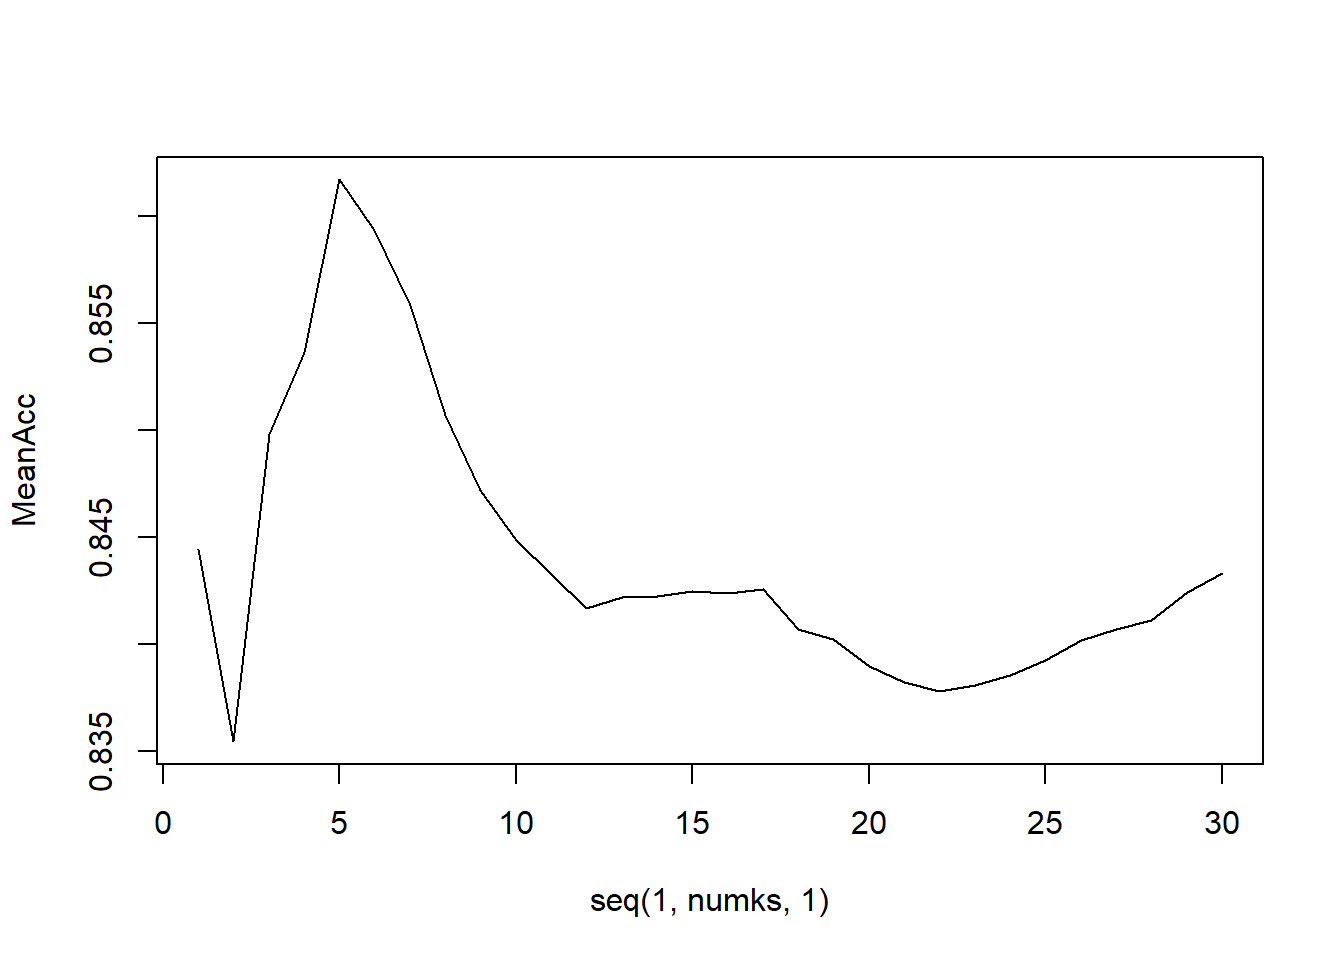
\includegraphics{Beer_Study_files/figure-latex/unnamed-chunk-15-1.pdf}

\textbf{Now that we know the optimum k value is 5, we run the KNN with
k=5.}

\textbf{We can see below that we can classify Ales and IPA's by their
ABV and IBU values with an accuracy of 87\%. We also created a NBB model
using the same dataset}

\begin{Shaded}
\begin{Highlighting}[]
\NormalTok{trainIndices =}\StringTok{ }\KeywordTok{sample}\NormalTok{(}\DecValTok{1}\OperatorTok{:}\KeywordTok{dim}\NormalTok{(dfAles)[}\DecValTok{1}\NormalTok{],}\KeywordTok{round}\NormalTok{(splitPerc }\OperatorTok{*}\StringTok{ }\KeywordTok{dim}\NormalTok{(dfAles)[}\DecValTok{1}\NormalTok{]))}
\NormalTok{train =}\StringTok{ }\NormalTok{dfAles[trainIndices,]}
\NormalTok{test =}\StringTok{ }\NormalTok{dfAles[}\OperatorTok{-}\NormalTok{trainIndices,]}

\CommentTok{# k = 5}
\NormalTok{classifications =}\StringTok{ }\KeywordTok{knn}\NormalTok{(train[,}\KeywordTok{c}\NormalTok{(}\StringTok{"ABV"}\NormalTok{, }\StringTok{"IBU"}\NormalTok{)],test[,}\KeywordTok{c}\NormalTok{(}\StringTok{"ABV"}\NormalTok{, }\StringTok{"IBU"}\NormalTok{)],train}\OperatorTok{$}\NormalTok{Ales, }\DataTypeTok{prob =} \OtherTok{TRUE}\NormalTok{, }\DataTypeTok{k =} \DecValTok{5}\NormalTok{)}
\KeywordTok{table}\NormalTok{(test}\OperatorTok{$}\NormalTok{Ales,classifications)}
\end{Highlighting}
\end{Shaded}

\begin{verbatim}
##      classifications
##       Ale IPA
##   Ale 120  13
##   IPA  17  86
\end{verbatim}

\begin{Shaded}
\begin{Highlighting}[]
\KeywordTok{confusionMatrix}\NormalTok{(}\KeywordTok{table}\NormalTok{(test}\OperatorTok{$}\NormalTok{Ales,classifications))}
\end{Highlighting}
\end{Shaded}

\begin{verbatim}
## Confusion Matrix and Statistics
## 
##      classifications
##       Ale IPA
##   Ale 120  13
##   IPA  17  86
##                                           
##                Accuracy : 0.8729          
##                  95% CI : (0.8235, 0.9126)
##     No Information Rate : 0.5805          
##     P-Value [Acc > NIR] : <2e-16          
##                                           
##                   Kappa : 0.7405          
##                                           
##  Mcnemar's Test P-Value : 0.5839          
##                                           
##             Sensitivity : 0.8759          
##             Specificity : 0.8687          
##          Pos Pred Value : 0.9023          
##          Neg Pred Value : 0.8350          
##              Prevalence : 0.5805          
##          Detection Rate : 0.5085          
##    Detection Prevalence : 0.5636          
##       Balanced Accuracy : 0.8723          
##                                           
##        'Positive' Class : Ale             
## 
\end{verbatim}

\begin{Shaded}
\begin{Highlighting}[]
\CommentTok{### NB model }

\NormalTok{model_}\DecValTok{2}\NormalTok{ =}\StringTok{ }\KeywordTok{naiveBayes}\NormalTok{(train[,}\KeywordTok{c}\NormalTok{(}\StringTok{"ABV"}\NormalTok{, }\StringTok{"IBU"}\NormalTok{)],train}\OperatorTok{$}\NormalTok{Ales)}
\NormalTok{table_cm =}\StringTok{ }\KeywordTok{table}\NormalTok{(}\KeywordTok{predict}\NormalTok{(model_}\DecValTok{2}\NormalTok{, test[,}\KeywordTok{c}\NormalTok{(}\StringTok{"ABV"}\NormalTok{, }\StringTok{"IBU"}\NormalTok{)]), test}\OperatorTok{$}\NormalTok{Ales)}
\NormalTok{CM =}\StringTok{ }\KeywordTok{confusionMatrix}\NormalTok{(table_cm)}
\NormalTok{CM}
\end{Highlighting}
\end{Shaded}

\begin{verbatim}
## Confusion Matrix and Statistics
## 
##      
##       Ale IPA
##   Ale 117  17
##   IPA  16  86
##                                           
##                Accuracy : 0.8602          
##                  95% CI : (0.8093, 0.9018)
##     No Information Rate : 0.5636          
##     P-Value [Acc > NIR] : <2e-16          
##                                           
##                   Kappa : 0.7154          
##                                           
##  Mcnemar's Test P-Value : 1               
##                                           
##             Sensitivity : 0.8797          
##             Specificity : 0.8350          
##          Pos Pred Value : 0.8731          
##          Neg Pred Value : 0.8431          
##              Prevalence : 0.5636          
##          Detection Rate : 0.4958          
##    Detection Prevalence : 0.5678          
##       Balanced Accuracy : 0.8573          
##                                           
##        'Positive' Class : Ale             
## 
\end{verbatim}

\textbf{Additional Insights:}

\textbf{Quetion of Interest: Is there a difference in the size of beer
and region the beer came from and do they effect ABV or IBU?}

\textbf{Answer}:

\textbf{We decided to run a two-way ANOVA on the size of the beer and
the region that the beer came from to determine if these two variables
have an effect on ABV or IBU. The regions were defined as ``Northeast'',
``Midwest'', ``South'' and ``West'', from the census regions of the
United States. Not enough beers came from Hawaii or Alaska, so the
Pacific region was excluded. The size of the beer was limited to
``12oz'' and ``16oz'' since other sizes also did not have enough beers.
Plots were run, and visually it looks like both size of the beer and
region do have an effect on both ABV and IBU, but there doesn't look
like there is an interaction term. Running our two-way ANOVA showed no
interaction term for IBU nor ABV, but both region and size of the beer
has an effect on both ABV and IBU. This means that the effects of the
size of the beer and region have on ABV and IBU are independent, thus we
can look at the differences in ABV and IBU in each region. Both ABV and
IBU are statistically larger in 16oz beers than 12oz beers. The only
statistically significant difference in region IBU is the 6.8 IBU
average difference between the West and Midwest regions. The only
statistically significant difference in region ABV is the 0.22\% average
ABV difference between the Midwest and Northeast regions.}

\begin{Shaded}
\begin{Highlighting}[]
\CommentTok{## Question 9: Data parsing + Box plots}
\NormalTok{dfFull}\OperatorTok{$}\NormalTok{Ounces =}\StringTok{ }\KeywordTok{as.factor}\NormalTok{(dfFull}\OperatorTok{$}\NormalTok{Ounces)}
\NormalTok{dfFull}\OperatorTok{$}\NormalTok{State =}\StringTok{ }\KeywordTok{as.character}\NormalTok{(dfFull}\OperatorTok{$}\NormalTok{State)}
\CommentTok{# Cut state into 4 regions}
\NormalTok{dfFull}\OperatorTok{$}\NormalTok{Region =}\StringTok{ }\KeywordTok{Recode}\NormalTok{(dfFull}\OperatorTok{$}\NormalTok{State, }\StringTok{"c('CT', 'ME', 'MA', 'NH', 'RI', 'VT', 'NJ', 'NY', 'PA') ='Northeast'; c('OH','IN','IL','MI','WI','MN','IA','MO','KS','NE','SD','ND') = 'MidWest'; c('TX','OK','AR','LA','MS','AL','TN','KY','WV','MD','DC','DE','VA','NC','SC', 'GA','FL') = 'South'; c('HI','AK') = 'Pacific'; c('NM','CO','WY','MT','ID','UT','AZ','NV','CA','OR','WA') = 'West'"}\NormalTok{)}
\NormalTok{dfFull}\OperatorTok{$}\NormalTok{Region =}\StringTok{ }\KeywordTok{as.factor}\NormalTok{(dfFull}\OperatorTok{$}\NormalTok{Region)}

\CommentTok{# Use only 12 and 16 ounce beers}
\NormalTok{dfFull =}\StringTok{ }\NormalTok{dfFull[dfFull}\OperatorTok{$}\NormalTok{Ounces }\OperatorTok{==}\StringTok{ }\DecValTok{12} \OperatorTok{|}\StringTok{ }\NormalTok{dfFull}\OperatorTok{$}\NormalTok{Ounces }\OperatorTok{==}\StringTok{ }\DecValTok{16}\NormalTok{,]}
\NormalTok{dfFull =}\StringTok{ }\NormalTok{dfFull[dfFull}\OperatorTok{$}\NormalTok{Region }\OperatorTok{!=}\StringTok{ 'Pacific'}\NormalTok{,]}
\CommentTok{# my summary for use with boxplots}
\NormalTok{mysummary<-}\ControlFlowTok{function}\NormalTok{(x)\{}
\NormalTok{  result<-}\KeywordTok{c}\NormalTok{(}\KeywordTok{length}\NormalTok{(x),}\KeywordTok{mean}\NormalTok{(x),}\KeywordTok{sd}\NormalTok{(x),}\KeywordTok{sd}\NormalTok{(x)}\OperatorTok{/}\KeywordTok{sqrt}\NormalTok{(}\KeywordTok{length}\NormalTok{(x)), }\KeywordTok{min}\NormalTok{(x), }\KeywordTok{max}\NormalTok{(x), }\KeywordTok{IQR}\NormalTok{(x))}
  \KeywordTok{names}\NormalTok{(result)<-}\KeywordTok{c}\NormalTok{(}\StringTok{"N"}\NormalTok{,}\StringTok{"Mean"}\NormalTok{,}\StringTok{"SD"}\NormalTok{,}\StringTok{"SE"}\NormalTok{, }\StringTok{"Min"}\NormalTok{, }\StringTok{"Max"}\NormalTok{, }\StringTok{"IQR"}\NormalTok{)}
  \KeywordTok{return}\NormalTok{(result)}
\NormalTok{\}}
\CommentTok{# Create boxplots for both ABV and IBU}
\NormalTok{dfABV =}\StringTok{ }\NormalTok{dfFull }\OperatorTok\StringTok{ }\KeywordTok{filter}\NormalTok{(}\OperatorTok{!}\KeywordTok{is.na}\NormalTok{(ABV))}
\KeywordTok{ggboxplot}\NormalTok{(dfABV, }\DataTypeTok{x=}\StringTok{"Region"}\NormalTok{, }\DataTypeTok{y=}\StringTok{"ABV"}\NormalTok{, }\DataTypeTok{color=}\StringTok{"Ounces"}\NormalTok{, }\DataTypeTok{pallette =} \KeywordTok{c}\NormalTok{(}\StringTok{"#00AFBB"}\NormalTok{, }\StringTok{"#E7B800"}\NormalTok{))}\OperatorTok{+}
\KeywordTok{ggtitle}\NormalTok{(}\StringTok{"ABV of 12oz and 16oz Cans For Each Region"}\NormalTok{)}
\end{Highlighting}
\end{Shaded}

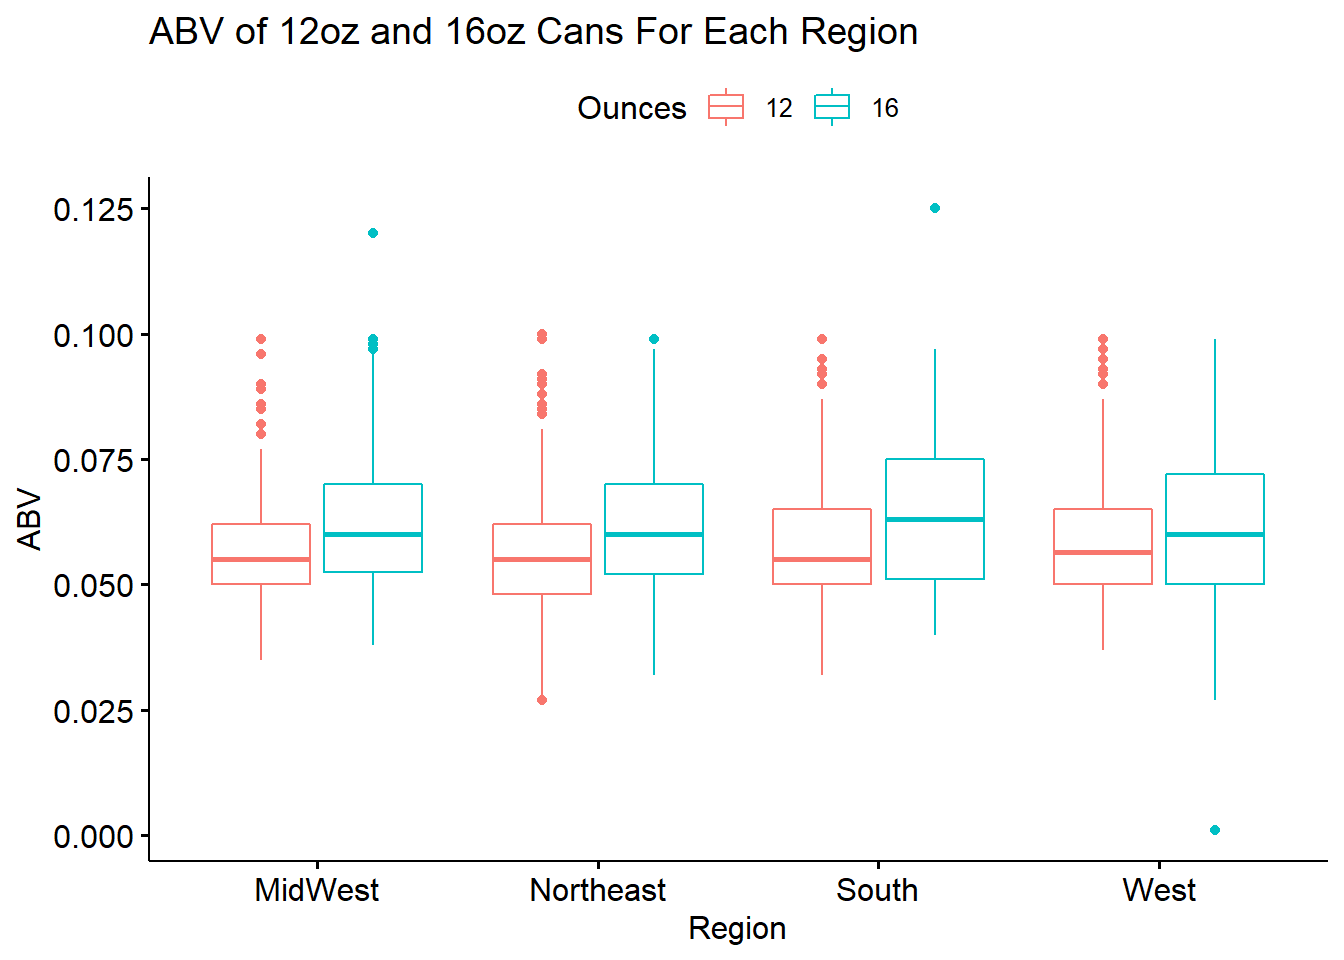
\includegraphics{Beer_Study_files/figure-latex/unnamed-chunk-18-1.pdf}

\begin{Shaded}
\begin{Highlighting}[]
\NormalTok{dfIBU =}\StringTok{ }\NormalTok{dfFull }\OperatorTok\StringTok{ }\KeywordTok{filter}\NormalTok{(}\OperatorTok{!}\KeywordTok{is.na}\NormalTok{(IBU))}
\KeywordTok{ggboxplot}\NormalTok{(dfIBU, }\DataTypeTok{x=}\StringTok{"Region"}\NormalTok{, }\DataTypeTok{y=}\StringTok{"IBU"}\NormalTok{, }\DataTypeTok{color=}\StringTok{"Ounces"}\NormalTok{, }\DataTypeTok{pallette =} \KeywordTok{c}\NormalTok{(}\StringTok{"#00AFBB"}\NormalTok{, }\StringTok{"#E7B800"}\NormalTok{))}\OperatorTok{+}
\KeywordTok{ggtitle}\NormalTok{(}\StringTok{"IBU of 12oz and 16oz Cans For Each Region"}\NormalTok{)}
\end{Highlighting}
\end{Shaded}

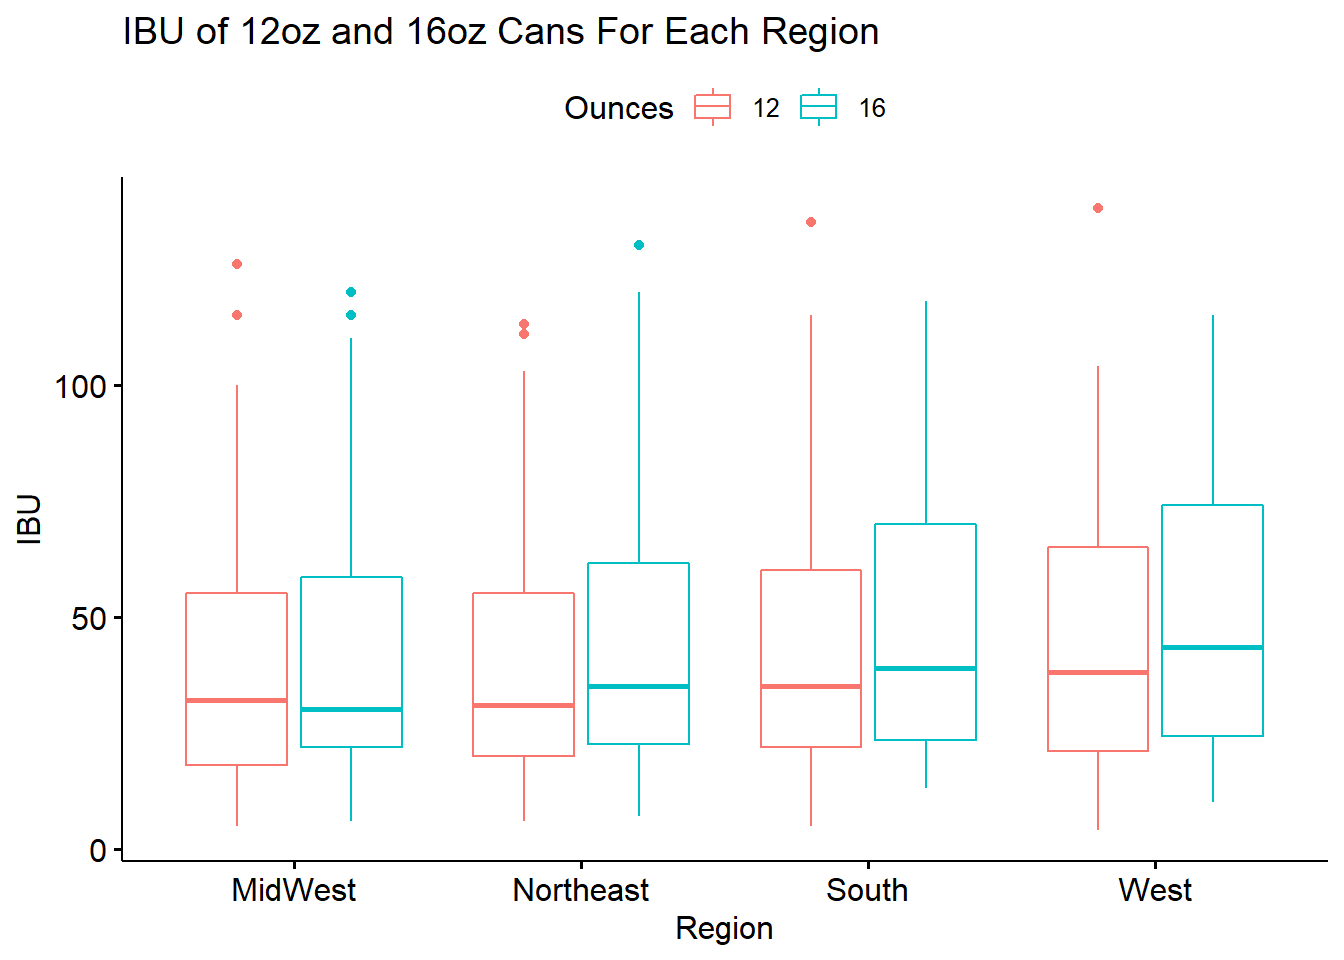
\includegraphics{Beer_Study_files/figure-latex/unnamed-chunk-18-2.pdf}

\begin{Shaded}
\begin{Highlighting}[]
\CommentTok{# Create line graphs with standard deviation bars}
\NormalTok{ABVsumstats<-}\KeywordTok{aggregate}\NormalTok{(ABV}\OperatorTok{~}\NormalTok{Region}\OperatorTok{*}\NormalTok{Ounces,}\DataTypeTok{data=}\NormalTok{dfABV,mysummary)}
\NormalTok{ABVsumstats<-}\KeywordTok{cbind}\NormalTok{(ABVsumstats[,}\DecValTok{1}\OperatorTok{:}\DecValTok{2}\NormalTok{],ABVsumstats[,}\OperatorTok{-}\NormalTok{(}\DecValTok{1}\OperatorTok{:}\DecValTok{2}\NormalTok{)])}

\KeywordTok{ggplot}\NormalTok{(ABVsumstats,}\KeywordTok{aes}\NormalTok{(}\DataTypeTok{x=}\NormalTok{Region,}\DataTypeTok{y=}\NormalTok{Mean,}\DataTypeTok{group=}\NormalTok{Ounces,}\DataTypeTok{colour=}\NormalTok{Ounces))}\OperatorTok{+}
\StringTok{  }\KeywordTok{ylab}\NormalTok{(}\StringTok{"ABV"}\NormalTok{)}\OperatorTok{+}
\StringTok{  }\KeywordTok{geom_line}\NormalTok{()}\OperatorTok{+}
\StringTok{  }\KeywordTok{geom_point}\NormalTok{()}\OperatorTok{+}
\StringTok{  }\KeywordTok{ggtitle}\NormalTok{(}\StringTok{"ABV of 12oz and 16oz Cans For Each Region"}\NormalTok{)}\OperatorTok{+}
\StringTok{  }\KeywordTok{geom_errorbar}\NormalTok{(}\KeywordTok{aes}\NormalTok{(}\DataTypeTok{ymin=}\NormalTok{Mean}\OperatorTok{-}\NormalTok{SD,}\DataTypeTok{ymax=}\NormalTok{Mean}\OperatorTok{+}\NormalTok{SD),}\DataTypeTok{width=}\NormalTok{.}\DecValTok{1}\NormalTok{)}
\end{Highlighting}
\end{Shaded}

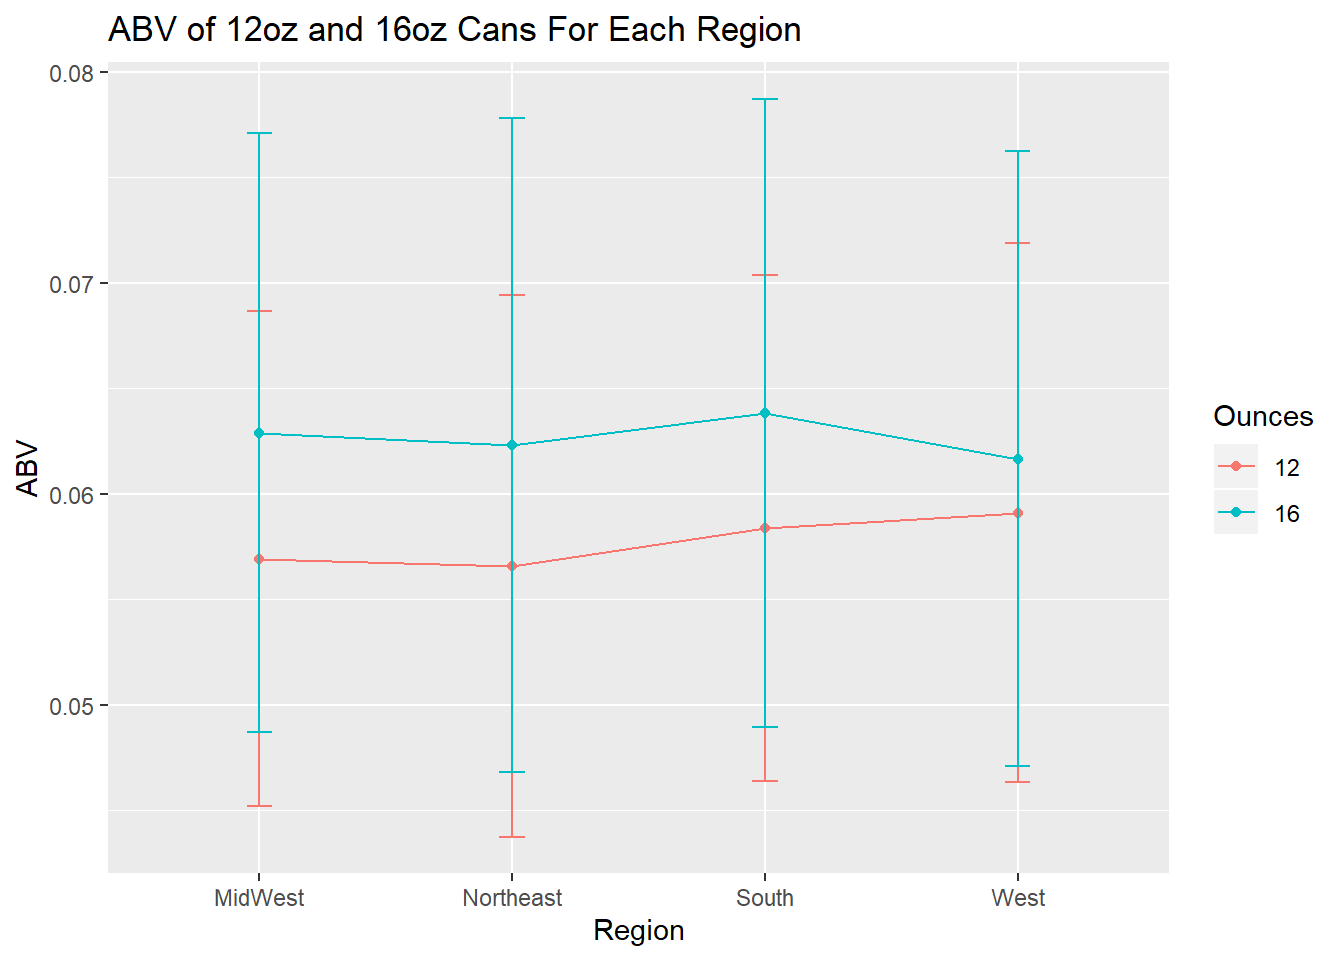
\includegraphics{Beer_Study_files/figure-latex/unnamed-chunk-19-1.pdf}

\begin{Shaded}
\begin{Highlighting}[]
\CommentTok{# Line graph with IBU}
\NormalTok{IBUsumstats<-}\KeywordTok{aggregate}\NormalTok{(IBU}\OperatorTok{~}\NormalTok{Region}\OperatorTok{*}\NormalTok{Ounces,}\DataTypeTok{data=}\NormalTok{dfIBU,mysummary)}
\NormalTok{IBUsumstats<-}\KeywordTok{cbind}\NormalTok{(IBUsumstats[,}\DecValTok{1}\OperatorTok{:}\DecValTok{2}\NormalTok{],IBUsumstats[,}\OperatorTok{-}\NormalTok{(}\DecValTok{1}\OperatorTok{:}\DecValTok{2}\NormalTok{)])}

\KeywordTok{ggplot}\NormalTok{(IBUsumstats,}\KeywordTok{aes}\NormalTok{(}\DataTypeTok{x=}\NormalTok{Region,}\DataTypeTok{y=}\NormalTok{Mean,}\DataTypeTok{group=}\NormalTok{Ounces,}\DataTypeTok{colour=}\NormalTok{Ounces))}\OperatorTok{+}
\StringTok{  }\KeywordTok{ylab}\NormalTok{(}\StringTok{"IBU"}\NormalTok{)}\OperatorTok{+}
\StringTok{  }\KeywordTok{geom_line}\NormalTok{()}\OperatorTok{+}
\StringTok{  }\KeywordTok{geom_point}\NormalTok{()}\OperatorTok{+}
\StringTok{  }\KeywordTok{ggtitle}\NormalTok{(}\StringTok{"IBU of 12oz and 16oz Cans For Each Region"}\NormalTok{)}\OperatorTok{+}
\StringTok{  }\KeywordTok{geom_errorbar}\NormalTok{(}\KeywordTok{aes}\NormalTok{(}\DataTypeTok{ymin=}\NormalTok{Mean}\OperatorTok{-}\NormalTok{SD,}\DataTypeTok{ymax=}\NormalTok{Mean}\OperatorTok{+}\NormalTok{SD),}\DataTypeTok{width=}\NormalTok{.}\DecValTok{1}\NormalTok{)}
\end{Highlighting}
\end{Shaded}

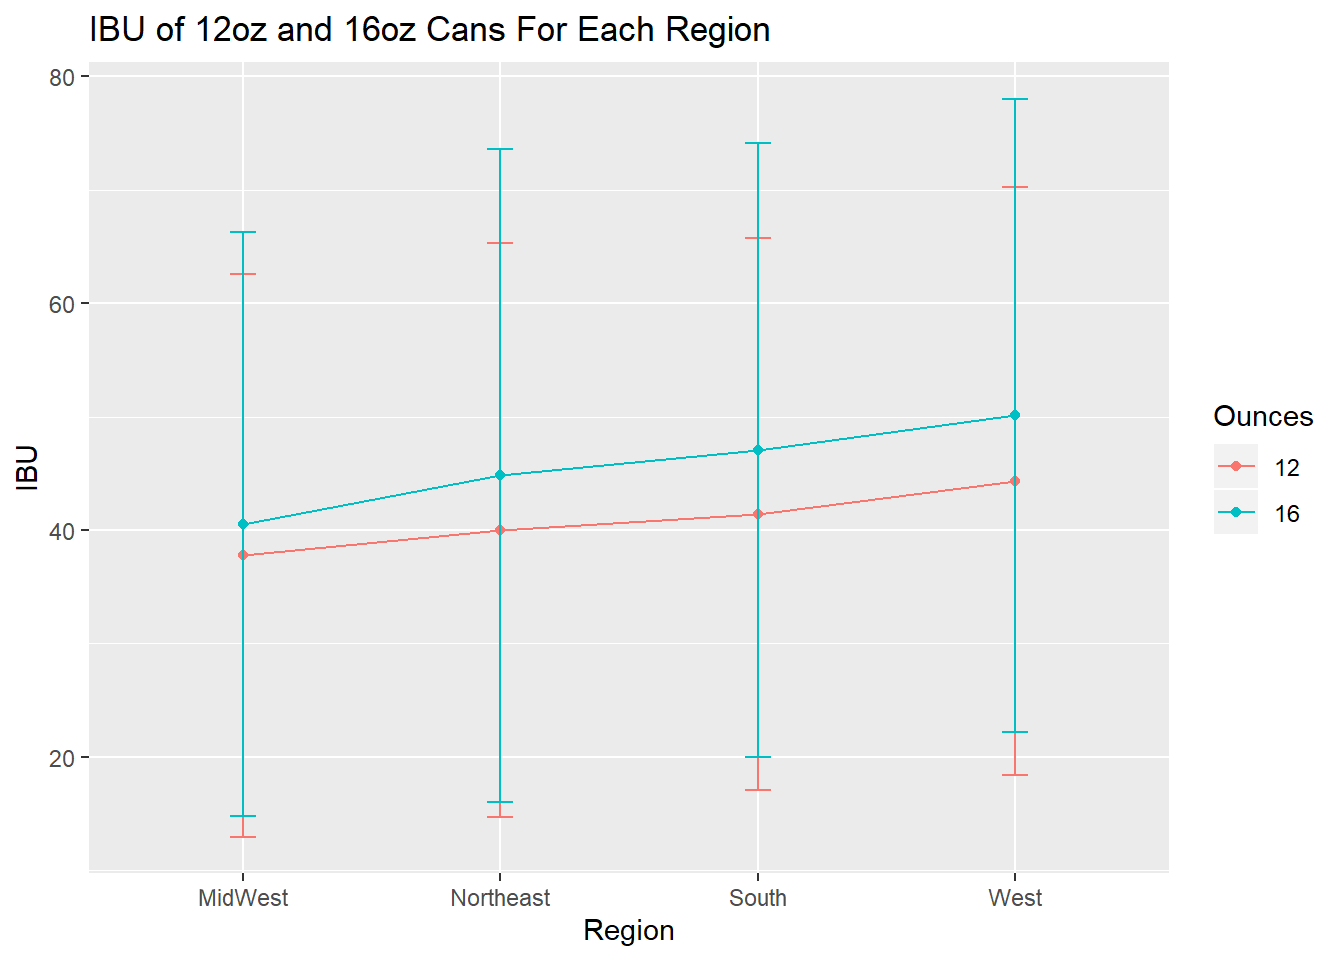
\includegraphics{Beer_Study_files/figure-latex/unnamed-chunk-20-1.pdf}

\begin{Shaded}
\begin{Highlighting}[]
\CommentTok{# Run two-way ANOVA}
\NormalTok{res.aov <-}\StringTok{ }\KeywordTok{aov}\NormalTok{(dfIBU}\OperatorTok{$}\NormalTok{IBU }\OperatorTok{~}\StringTok{ }\NormalTok{dfIBU}\OperatorTok{$}\NormalTok{Region }\OperatorTok{+}\StringTok{ }\NormalTok{dfIBU}\OperatorTok{$}\NormalTok{Ounces }\OperatorTok{+}\StringTok{ }\NormalTok{dfIBU}\OperatorTok{$}\NormalTok{Region}\OperatorTok{:}\NormalTok{dfIBU}\OperatorTok{$}\NormalTok{Ounces)}
\KeywordTok{summary}\NormalTok{(res.aov)}
\end{Highlighting}
\end{Shaded}

\begin{verbatim}
##                             Df Sum Sq Mean Sq F value  Pr(>F)   
## dfIBU$Region                 3  10248    3416   5.108 0.00162 **
## dfIBU$Ounces                 1   6241    6241   9.332 0.00230 **
## dfIBU$Region:dfIBU$Ounces    3    504     168   0.251 0.86054   
## Residuals                 1344 898819     669                   
## ---
## Signif. codes:  0 '***' 0.001 '**' 0.01 '*' 0.05 '.' 0.1 ' ' 1
\end{verbatim}

\begin{Shaded}
\begin{Highlighting}[]
\CommentTok{#IBU comparisons}
\KeywordTok{TukeyHSD}\NormalTok{(res.aov)}
\end{Highlighting}
\end{Shaded}

\begin{verbatim}
##   Tukey multiple comparisons of means
##     95% family-wise confidence level
## 
## Fit: aov(formula = dfIBU$IBU ~ dfIBU$Region + dfIBU$Ounces + dfIBU$Region:dfIBU$Ounces)
## 
## $`dfIBU$Region`
##                       diff        lwr       upr     p adj
## Northeast-MidWest 2.189423 -3.6178264  7.996672 0.7666943
## South-MidWest     3.372305 -1.8936125  8.638222 0.3524380
## West-MidWest      6.777855  2.2158294 11.339881 0.0007983
## South-Northeast   1.182882 -4.9490317  7.314795 0.9599376
## West-Northeast    4.588433 -0.9507517 10.127617 0.1438849
## West-South        3.405551 -1.5631816  8.374283 0.2917708
## 
## $`dfIBU$Ounces`
##           diff      lwr      upr     p adj
## 16-12 4.338582 1.452593 7.224571 0.0032419
## 
## $`dfIBU$Region:dfIBU$Ounces`
##                                 diff         lwr       upr     p adj
## Northeast:12-MidWest:12    2.2466132  -6.7318191 11.225045 0.9950075
## South:12-MidWest:12        3.6523650  -4.4206699 11.725400 0.8693574
## West:12-MidWest:12         6.5642336  -0.8258389 13.954306 0.1244475
## MidWest:16-MidWest:12      2.7787366  -5.4135772 10.971050 0.9699606
## Northeast:16-MidWest:12    7.0621016  -4.6128908 18.737094 0.5952680
## South:16-MidWest:12        9.2879081  -2.3870843 20.962900 0.2347489
## West:16-MidWest:12        12.3461876   3.5150082 21.177367 0.0006179
## South:12-Northeast:12      1.4057518  -7.0782815  9.889785 0.9996489
## West:12-Northeast:12       4.3176204  -3.5193498 12.154591 0.7052216
## MidWest:16-Northeast:12    0.5321235  -8.0654887  9.129736 0.9999996
## Northeast:16-Northeast:12  4.8154884  -7.1473865 16.778363 0.9255115
## South:16-Northeast:12      7.0412949  -4.9215800 19.004170 0.6292341
## West:16-Northeast:12      10.0995745   0.8911728 19.307976 0.0201093
## West:12-South:12           2.9118686  -3.8689682  9.692705 0.8976759
## MidWest:16-South:12       -0.8736284  -8.5208881  6.773631 0.9999714
## Northeast:16-South:12      3.4097366  -7.8894679 14.708941 0.9845751
## South:16-South:12          5.6355431  -5.6636614 16.934748 0.8000173
## West:16-South:12           8.6938226   0.3657793 17.021866 0.0335186
## MidWest:16-West:12        -3.7854970 -10.7079143  3.136920 0.7131523
## Northeast:16-West:12       0.4978680 -10.3239296 11.319666 0.9999999
## South:16-West:12           2.7236745  -8.0981231 13.545472 0.9948246
## West:16-West:12            5.7819540  -1.8858740 13.449782 0.3002933
## Northeast:16-MidWest:16    4.2833650  -7.1013676 15.668098 0.9473743
## South:16-MidWest:16        6.5091714  -4.8755612 17.893904 0.6637771
## West:16-MidWest:16         9.5674510   1.1237302 18.011172 0.0139018
## South:16-Northeast:16      2.2258065 -11.8739658 16.325579 0.9997456
## West:16-Northeast:16       5.2840860  -6.5686715 17.136844 0.8779194
## West:16-South:16           3.0582796  -8.7944780 14.911037 0.9939680
\end{verbatim}

\begin{Shaded}
\begin{Highlighting}[]
\CommentTok{# ABV two-way ANOVA}
\NormalTok{res.aov2 <-}\StringTok{ }\KeywordTok{aov}\NormalTok{(dfABV}\OperatorTok{$}\NormalTok{ABV }\OperatorTok{~}\StringTok{ }\NormalTok{dfABV}\OperatorTok{$}\NormalTok{Region }\OperatorTok{+}\StringTok{ }\NormalTok{dfABV}\OperatorTok{$}\NormalTok{Ounces }\OperatorTok{+}\StringTok{ }\NormalTok{dfABV}\OperatorTok{$}\NormalTok{Region}\OperatorTok{:}\NormalTok{dfABV}\OperatorTok{$}\NormalTok{Ounces)}
\KeywordTok{summary}\NormalTok{(res.aov2)}
\end{Highlighting}
\end{Shaded}

\begin{verbatim}
##                             Df Sum Sq  Mean Sq F value   Pr(>F)    
## dfABV$Region                 3 0.0013 0.000436   2.497   0.0581 .  
## dfABV$Ounces                 1 0.0102 0.010172  58.259 3.37e-14 ***
## dfABV$Region:dfABV$Ounces    3 0.0012 0.000392   2.244   0.0812 .  
## Residuals                 2249 0.3927 0.000175                     
## ---
## Signif. codes:  0 '***' 0.001 '**' 0.01 '*' 0.05 '.' 0.1 ' ' 1
\end{verbatim}

\begin{Shaded}
\begin{Highlighting}[]
\CommentTok{#ABV Comparisons}
\KeywordTok{TukeyHSD}\NormalTok{(res.aov2)}
\end{Highlighting}
\end{Shaded}

\begin{verbatim}
##   Tukey multiple comparisons of means
##     95% family-wise confidence level
## 
## Fit: aov(formula = dfABV$ABV ~ dfABV$Region + dfABV$Ounces + dfABV$Region:dfABV$Ounces)
## 
## $`dfABV$Region`
##                            diff           lwr           upr     p adj
## Northeast-MidWest -0.0022313511 -0.0044219435 -4.075864e-05 0.0439941
## South-MidWest     -0.0008677869 -0.0029701982  1.234624e-03 0.7132219
## West-MidWest      -0.0003533624 -0.0021367495  1.430025e-03 0.9568696
## South-Northeast    0.0013635641 -0.0010467200  3.773848e-03 0.4654744
## West-Northeast     0.0018779887 -0.0002597218  4.015699e-03 0.1081968
## West-South         0.0005144246 -0.0015328282  2.561677e-03 0.9169622
## 
## $`dfABV$Ounces`
##              diff         lwr         upr p adj
## 16-12 0.004219831 0.003085776 0.005353885     0
## 
## $`dfABV$Region:dfABV$Ounces`
##                                    diff           lwr         upr     p adj
## Northeast:12-MidWest:12   -0.0003454599 -3.705236e-03 0.003014316 0.9999862
## South:12-MidWest:12        0.0014538387 -1.732193e-03 0.004639870 0.8646078
## West:12-MidWest:12         0.0021797918 -7.412543e-04 0.005100838 0.3142254
## MidWest:16-MidWest:12      0.0059625584  2.854263e-03 0.009070854 0.0000002
## Northeast:16-MidWest:12    0.0053737990  6.799414e-04 0.010067657 0.0122578
## South:16-MidWest:12        0.0069040982  1.897827e-03 0.011910370 0.0007803
## West:16-MidWest:12         0.0047259927  1.306300e-03 0.008145685 0.0007515
## South:12-Northeast:12      0.0017992986 -1.442192e-03 0.005040789 0.6977894
## West:12-Northeast:12       0.0025252517 -4.561870e-04 0.005506690 0.1676488
## MidWest:16-Northeast:12    0.0063080183  3.142901e-03 0.009473136 0.0000000
## Northeast:16-Northeast:12  0.0057192589  9.875821e-04 0.010450936 0.0061223
## South:16-Northeast:12      0.0072495581  2.207810e-03 0.012291306 0.0003583
## West:16-Northeast:12       0.0050714526  1.600032e-03 0.008542874 0.0002619
## West:12-South:12           0.0007259531 -2.058231e-03 0.003510137 0.9936040
## MidWest:16-South:12        0.0045087197  1.528674e-03 0.007488765 0.0001265
## Northeast:16-South:12      0.0039199603 -6.899712e-04 0.008529892 0.1638077
## South:16-South:12          0.0054502595  5.225903e-04 0.010377929 0.0182879
## West:16-South:12           0.0032721540 -3.139981e-05 0.006575708 0.0543635
## MidWest:16-West:12         0.0037827666  1.087885e-03 0.006477648 0.0005658
## Northeast:16-West:12       0.0031940072 -1.236928e-03 0.007624942 0.3600238
## South:16-West:12           0.0047243065 -3.632772e-05 0.009484941 0.0534787
## West:16-West:12            0.0025462010 -5.025991e-04 0.005595001 0.1817970
## Northeast:16-MidWest:16   -0.0005887594 -5.145312e-03 0.003967794 0.9999343
## South:16-MidWest:16        0.0009415398 -3.936229e-03 0.005819309 0.9990479
## West:16-MidWest:16        -0.0012365657 -4.465215e-03 0.001992083 0.9424912
## South:16-Northeast:16      0.0015302992 -4.483304e-03 0.007543903 0.9944921
## West:16-Northeast:16      -0.0006478063 -5.422214e-03 0.004126602 0.9999085
## West:16-South:16          -0.0021781055 -7.259978e-03 0.002903767 0.8989944
\end{verbatim}

\end{document}
